%%%%%%%%%%%%%%%%%%%%%%%%%%%%%%%%%%%%%%%%%%%%%%%%%%%%%%%%%%%%%%%%%%%%%%%%%%%

\documentclass[a4paper,oneside,12pt]{article}
\usepackage{mystyle}

\begin{document}

\title{\Large\bf Exponential functions}
\author{%%
  Minh Van Nguyen \\
  \url{mvngu@gmx.com}
}
\date{\today}
\maketitle


%%%%%%%%%%%%%%%%%%%%%%%%%%%%%%%%%%%%%%%%%%%%%%%%%%%%%%%%%%%%%%%%%%%%%%%%%%%

\section{An example}

Exponential functions are commonly used to understand the change in a
population over time.  The population can be the residents of a
country, the ants in an ant colony, the bacteria in a Petri dish, or
the amount of carbon-14 in the bone of an animal that lived thousands
of years ago.  In particular, what you want to know is the
\emph{percentage rate} of change over time, where time can be measured
in terms of seconds, minutes, hours, days, months, or years.  If you
know the \emph{initial population} and the percentage rate of change,
then you can use the exponential function to calculate the population
in the next year or the next three years.  The following example
should help you to understand the ideas presented above.\footnote{
  The following video explains the idea of exponential growth in terms
  of folding a piece of paper:
  \url{https://youtu.be/AmFMJC45f1Q}.
  The next video uses many more examples to explain exponential
  growth:
  \url{https://youtu.be/0BSaMH4hINY}.
  For an explanation of the growth rate, growth factor, decay rate,
  and decay factor see this video:
  \url{https://youtu.be/VrkQKiCqryk}.
}

\begin{example}
\label{eg:Australian_population_2017}
\textbf{Population of Australia.}
According to the Australian Bureau of Statistics~(ABS), at the end of
September 2017 the population of Australia grew by $1.6\%$ since the
previous year.\footnote{
  ``3101.0 - Australian Demographic Statistics, Sep 2017'',
  \url{http://web.archive.org/web/20180420062713/http://www.abs.gov.au/AUSSTATS/abs@.nsf/Lookup/3101.0Main+Features1Sep\%202017},
  accessed 2018-04-20.
}
The population by the end of the given period was estimated to be
$24.7029$ million people.  Assume that for the next few years the
population of Australia will grow by a rate of $1.6\%$ per annum.
%%
\begin{packedenum}
\item\label{subeg:Australian_population_2017_growth_rate}
  Identify the rate of change.

\item\label{subeg:Australian_population_2017_initial_population}
  Determine the initial population.

\item\label{subeg:Australian_population_2017_table_graph}
  Provide a table of values for the projected population of Australia
  from 2017 to 2021, inclusive.  Graph the data in the table as a
  scatter plot.
\end{packedenum}
\end{example}

\begin{solution}
\solutionpart{subeg:Australian_population_2017_growth_rate}
By the end of September 2017, the population of Australia grew by
$1.6\%$ from the previous year so the percentage rate of change is
$1.6\%$.  Since you are concerned with population growth, the rate of
change in this example is also called the \emph{growth rate}.  The
growth rate can be written as a percentage or as a fraction.  To
express the percentage of $1.6\%$ as a fraction, you divide the number
$1.6$ by $100$ to get the decimal representation
\[
\frac{1.6}{100}
=
0.016.
\]
That is, you can also say that the growth rate is $0.016$ per annum.

\solutionpart{subeg:Australian_population_2017_initial_population}
The example does not explicitly state the value of the initial
population.  However, the example does say that the population of
Australia by the end of September 2017 was $24.7029$ million people so
you can consider this number as the initial population.  The reason
why you require an initial population is so that the population can
grow or decline.  You need to start somewhere.

\solutionpart{subeg:Australian_population_2017_table_graph}
You are required to predict the population of Australia from $2018$ to
$2021$, inclusive.  To calculate the projected~(or predicted)
population in $2018$, you must know two numbers: the population in
$2017$ and the growth rate.
From \Part{subeg:Australian_population_2017_growth_rate} you know that
the growth rate is $0.016$ per annum and
from \Part{subeg:Australian_population_2017_initial_population} you
know that the population of Australia for 2017 was $24.7029$ million
people.  By $2018$, the population would have increased by
%%
\begin{equation}
\label{eqn:Australian_population_2018}
24.7029 \times 0.016
=
0.3952464
\end{equation}
%%
million people.  To calculate the population for $2018$, you must add
the number in~\eqref{eqn:Australian_population_2018} to the population
in $2017$.  The projected population for $2018$ is given by the
expression $24.7029 + 24.7029 \times 0.016$.  Factoring out the number
$24.7029$ and simplifying shows that the required population number is
%%
\begin{equation}
\label{eqn:Australian_population_2018_calculation}
\begin{aligned}
&24.7029 + 24.7029 \times 0.016 \\[4pt]
&=
24.7029 (1 + 0.016) \\[4pt]
&=
24.7029 \times 1.016 \\[4pt]
&=
25.0981464
\end{aligned}
\end{equation}
%%
million people.

Now use the same technique as explained above to calculate the
projected population for $2019$.  You already know that the growth
rate is $0.016$ per annum and that the population in $2018$ would be
$25.0981464$ million people.  By $2019$, the population would have
increased by
%%
\begin{equation}
\label{eqn:Australian_population_2019}
25.0981464 \times 0.016
=
0.4015703424
\end{equation}
%%
million people.  The projected population for $2019$ is the number
in~\eqref{eqn:Australian_population_2019} added to the population in
$2018$.  By $2019$ Australia is projected to have a population of
%%
\begin{align*}
&25.0981464 + 25.0981464 \times 0.016 \\[4pt]
&=
25.0981464 (1 + 0.016) \\[4pt]
&=
25.0981464 \times 1.016 \\[4pt]
&=
25.4997167424
\end{align*}
%%
million people.  Use the same technique as explained above to
calculate the projected population in $2020$ and $2021$.  The
projected populations through to the year $2021$ are shown in
\Table{tab:Australian_population_2017}, a graph of which is
illustrated in \Figure{fig:Australian_population_2017}.
\end{solution}

\begin{table}[!htbp]
\centering
\begin{tabular}{cl}           \toprule
Year   & Population         \\\midrule
$2017$ & $24.7029$          \\[4pt]
$2018$ & $25.0981464$       \\[4pt]
$2019$ & $25.4997167424$    \\[4pt]
$2020$ & $25.9077122102784$ \\[4pt]
$2021$ & $26.3222356056429$ \\\bottomrule
\end{tabular}

\caption{%%
  The projected population of Australia through to the year $2021$.
  The population numbers are in terms of millions.  For example, the
  population in $2017$ was estimated to be $24.7029$ million people.
  The population is assumed to grow at a rate of $1.6\%$ per annum.
}
\label{tab:Australian_population_2017}
\end{table}

\begin{figure}[!htbp]
\centering
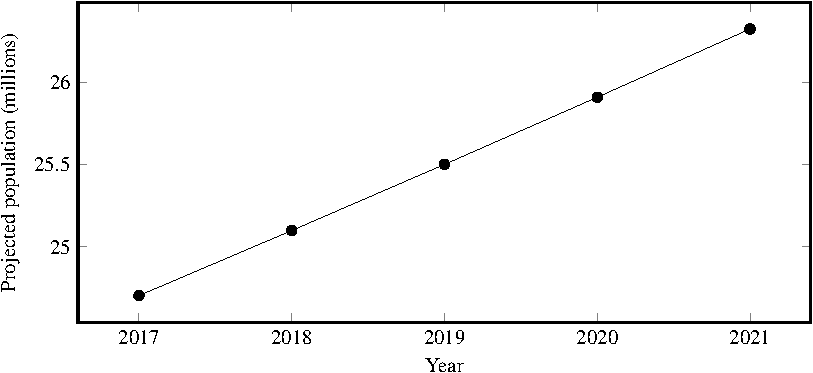
\includegraphics[scale=1.1]{image/11/australian-population.pdf}
\caption{%%
  The projected population~(in millions) of Australia through to the
  year $2021$.  The population is assumed to grow at a rate of $1.6\%$
  per annum.  Data are from \Table{tab:Australian_population_2017}.
}
\label{fig:Australian_population_2017}
\end{figure}

The next question you might ask is:  Is there a formula to calculate
the population of Australia for any number of years since $2017$?  The
answer is yes, but you must assume that the population grows by a
constant percentage rate each year.  Assume that you have an initial
population of $24.7029$ million people in $2017$ and that the growth
rate is $1.6\%$ or $0.016$ per annum.  According to
\Equation{eqn:Australian_population_2018_calculation}, in
$2018$~(i.e.~one year from $2017$) the population can be written as
the expression
\[
24.7029 + 24.7029 \times 0.016
=
24.7029 \times 1.016.
\]
In $2019$~(i.e.~two years from $2017$) the population can be written
as
%%
\begin{align*}
&24.7029 \times 1.016 + 24.7029 \times 1.016 \times 0.016 \\[4pt]
&=
24.7029 \times 1.016 (1 + 0.016) \\[4pt]
&=
24.7029 \times 1.016 \times 1.016 \\[4pt]
&=
24.7029 \times 1.016^2.
\end{align*}
%%
In $2020$~(i.e.~three years from $2017$) the population can be written
as
%%
\begin{align*}
&24.7029 \times 1.016^2 + 24.7029 \times 1.016^2 \times 0.016 \\[4pt]
&=
24.7029 \times 1.016^2 (1 + 0.016) \\[4pt]
&=
24.7029 \times 1.016^2 \times 1.016 \\[4pt]
&=
24.7029 \times 1.016^3.
\end{align*}
%%
In $2021$~(i.e.~four years from $2017$) the population can be written
as
%%
\begin{align*}
&24.7029 \times 1.016^3 + 24.7029 \times 1.016^3 \times 0.016 \\[4pt]
&=
24.7029 \times 1.016^3 (1 + 0.016) \\[4pt]
&=
24.7029 \times 1.016^3 \times 1.016 \\[4pt]
&=
24.7029 \times 1.016^4.
\end{align*}
%%
From the above equations, you can see that the only number that
changes is the exponent or power of $1.016$.  If $t$ is the number of
years since $2017$, then the population~(in millions) in $t$ years
since $2017$ can be written as
%%
\begin{equation}
\label{eqn:Australian_population_formula}
24.7029 \times 1.016^t.
\end{equation}
%%
You can see from \Expression{eqn:Australian_population_formula} that
the initial population is $24.7029$ million people.  The number
$1.016$ is called the \emph{growth factor} and can be written in terms
of the growth rate as $1.016 = 1 + 0.016$.

\begin{exercise}
Use \Expression{eqn:Australian_population_formula} to verify the
population numbers in \Table{tab:Australian_population_2017}.
\end{exercise}

\ifbool{showSolution}{
\begin{solution}
In \Table{tab:Australian_population_2017}, the year $2017$ is $t = 0$
years since $2017$ so according to
\Expression{eqn:Australian_population_formula} the population in
$2017$ is
\[
24.7029 \times 1.016^0
=
24.7029
\]
million people.  The year $2018$ is $t = 1$ year since $2017$ so the
population in $2018$ is
\[
24.7029 \times 1.016^1
=
25.0981464
\]
million people.  The year $2019$ is $t = 2$ years since $2017$ so the
population in $2019$ is
\[
24.7029 \times 1.016^2
=
25.4997167424
\]
million people.  The year $2020$ is $t = 3$ years since $2017$ so the
population in $2020$ is approximately
\[
24.7029 \times 1.016^3
=
25.9077122102784
\]
million people.  Finally, the year $2021$ is $t = 4$ years since
$2017$ so the population in $2021$ is approximately
\[
24.7029 \times 1.016^4
=
26.3222356056429
\]
million people.
\end{solution}
}{}


%%%%%%%%%%%%%%%%%%%%%%%%%%%%%%%%%%%%%%%%%%%%%%%%%%%%%%%%%%%%%%%%%%%%%%%%%%%

\section{Exponential growth}
\label{sec:exponential_growth}

Let's derive a general formula to model situations such as those
presented in \Example{eg:Australian_population_2017}.  Denote by $a$
the initial value of the population and assume that $a \neq 0$.  Let
$r$ be the decimal representation of the percentage rate of change and
define the growth factor by $b = 1 + r$.  For example, if the
population grows by a constant percentage of $2.3\%$, the decimal
representation of this percentage rate of change is
$r = 2.3 / 100 = 0.023$ and the growth factor is
$b = 1 + 0.023 = 1.023$.  The amount of time since the initial
population is represented by $t$.  So you assume that $t \geq 0$ and
at time $t = 0$ you have the initial population of $a$.  At time
$t = 1$, the population would have changed by an amount of $ar$ since
time $t = 0$.  You add this number to the population at time $t = 0$
to get the population at $t = 1$.  Then the population at time $t = 1$
is given by
\[
a + ar
=
a(1 + r)
=
ab.
\]
At time $t = 2$, the population would have changed by an amount of
$abr$ since time $t = 1$.  You add this number to the population at
time $t = 1$ to get the population at time $t = 2$.  That is, the
population at time $t = 2$ is given by
\[
ab + abr
=
ab(1 + r)
=
abb
=
ab^2.
\]
Now you use the same technique as explained above to obtain the
population at time $t = 3$.  At time $t = 3$, the population would
have changed by an amount of $ab^2r$ since time $t = 2$.  Adding this
number to the population at time $t = 2$ shows that the population at
time $t = 3$ is given by
\[
ab^2 + ab^2r
=
ab^2 (1 + r)
=
ab^2b
=
ab^3.
\]
Use the same technique as explained above to see that the population
at time $t = 4$ is given by the expression
\[
ab^3 + ab^3r
=
ab^3 (1 + r)
=
ab^3b
=
ab^4.
\]
From the above equations, you see that in general the population
$Q(t)$ at time $t \geq 0$ is given by the formula
%%
\begin{equation}
\label{eqn:exponential_growth}
\begin{aligned}
Q(t)
&=
a(1 + r)^t \\[4pt]
&=
ab^t.
\end{aligned}
\end{equation}
%%
The above discussion is summarised in
\Theorem{thm:exponential_growth}.
\Figure{fig:general_exponential_growth} shows a general graph of what
an exponential growth looks like.

\begin{figure}[!htbp]
\centering
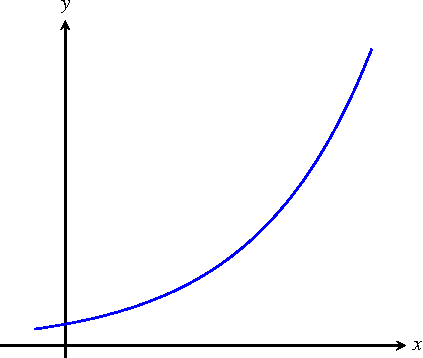
\includegraphics[scale=1.1]{image/11/exponential-growth.pdf}
\caption{%%
  The general graph of an exponential growth.
}
\label{fig:general_exponential_growth}
\end{figure}

\begin{theorem}
\label{thm:exponential_growth}
\textbf{Exponential growth.}
Let $a \neq 0$ be the initial value of a population.  Assume that the
population increases by a constant decimal rate of $r$ per unit time.
If $b = 1 + r$ is the growth factor and $Q(t)$ represents the
population number at time $t$, then $Q(t) = ab^t$.
\end{theorem}

One of the important ideas in exponential growth is the concept of
\emph{doubling time}.  You can think of the doubling time of a
population as the amount of time required for the initial population
number to double.  For example, suppose a Petri dish has five cells of
a type of bacteria and after $30$ minutes the number of bacteria cells
has doubled to ten cells.  Then the doubling time for the bacteria is
$30$ minutes.  In other words, every $30$ minutes the bacteria
population would have increased by $100\%$.  How can the doubling time
be calculated?

You can calculate a rough estimate of the doubling time of a
population by using a rule of thumb called the \emph{rule of 72}.  If
$p$ is the constant percentage rate of growth of a population, the
rule of $72$ states that a rough estimate of the doubling time of the
population is given by the ratio $72 / p$.  For instance, suppose that
a type of bacteria has a constant percentage rate of growth of $10\%$ per
hour and the initial population is $20$ bacteria cells.  Then $p = 10$
and the rule of $72$ tells you that the doubling time of the
population is roughly $72 / 10 = 7.2$ hours.  That is, after $7.2$
hours have elapsed you should expect the bacteria population to have
increased from the initial number of $20$ cells to $40$ cells.

\begin{theorem}
\textbf{Rule of 72.}
Let $p$ be the constant percentage rate of growth of a population.
Then the doubling time of the population is approximately $72 / p$
units of time.
\end{theorem}

Another way to determine the doubling time of a population is to use
the formula for the growth of the population.  In fact, you can first
use the rule of $72$ to produce a rough estimate of the doubling
time.  Then substitute the resulting doubling time into the formula to
see whether the rule of $72$ gives you a good estimate of the doubling
time of the population.  Going back to the example of bacterial growth
above, where the initial bacteria population is $a = 20$ cells and the
population is assumed to grow at a constant percentage rate of $10\%$
per hour.  The growth rate is $r = 0.1$ per hour and the growth factor
is $b = 1 + 0.1 = 1.1$.  Let $Q(t)$ represent the number of bacteria
cells after $t$ hours have elapsed.  Then the bacteria population can
be described by the formula $Q(t) = 20 \times 1.1^t$.  The rule of
$72$ yields the doubling time of $72 / 10 = 7.2$ hours.  Substitute
this result into the formula to get
\[
Q(7.2)
=
20 \times 1.1^{7.2}
\approx
39.7244
\]
rounded to four decimal places, not quite $40$ cells yet.  In fact,
after $t = 8$ hours have elapsed the number of bacteria cells would be
\[
Q(8)
=
20 \times 1.1^8
\approx
42.8718
\]
which is a little over $40$ cells.  You can conclude that the doubling
time of the bacteria population is roughly $7.2$ hours and at most $8$
hours.  The time of $8$ hours is an upper bound~(or upper limit) on
the doubling time.

\begin{example}
\label{eg:bacterial_growth}
\textbf{Bacterial growth.}
A Petri dish initially contains ten cells of a type of bacteria.  The
bacteria population is known to have a constant percentage growth rate
of $56\%$ per hour.
%%
\begin{packedenum}
\item\label{subeg:bacteria_growth_rate}
  Determine the growth rate and growth factor of the bacteria
  population.

\item\label{subeg:bacteria_initial_population}
  Determine the initial population of bacteria in the Petri dish.

\item\label{subeg:bacteria_growth_1_2_hours}
  Use the same technique as in
  \Expression{eqn:Australian_population_2018_calculation} to calculate
  the number of bacteria cells in the Petri dish after one hour.  How
  many bacteria cells would there be in the Petri dish after two
  hours?

\item\label{subeg:bacteria_growth_formula}
  Derive a formula for the number of bacteria cells in the Petri dish
  after $t$ hours have elapsed.  Use the formula to verify your
  results from \Part{subeg:bacteria_growth_1_2_hours}.  Produce a
  graph of the growth of the bacteria population after the elapse of
  at most $24$ hours.
\end{packedenum}
\end{example}

\begin{solution}
\solutionpart{subeg:bacteria_growth_rate}
Since the bacteria population grows at a constant percentage rate of
$56\%$ per hour, the growth rate is $r = 56 / 100 = 0.56$ per hour and
hence the growth factor is $b = 1 + 0.56 = 1.56$.

\solutionpart{subeg:bacteria_initial_population}
The initial population of bacteria is $a = 10$ cells.

\solutionpart{subeg:bacteria_growth_1_2_hours}
You have an initial bacteria population of $10$ cells.  At time
$t = 1$ hour, the bacteria population would have increased by
$10 \times 0.56$ cells.  Add this number to the initial population to
see that after one hour the bacteria population would be
%%
\begin{align*}
10 + 10 \times 0.56
&=
10 (1 + 0.56) \\[4pt]
&=
10 \times 1.56 \\[4pt]
&=
15.6
\end{align*}
%%
cells.  After two hours, the bacteria population would have increased
by $15.6 \times 0.56$ cells.  Adding this number to the population at
time $t = 1$ hour and you have
%%
\begin{align*}
15.6 + 15.6 \times 0.56
&=
15.6 (1 + 0.56) \\[4pt]
&=
15.6 \times 1.56 \\[4pt]
&=
24.336
\end{align*}
%%
cells at time $t = 2$ hours.

\solutionpart{subeg:bacteria_growth_formula}
From \Parts{subeg:bacteria_growth_rate}{subeg:bacteria_initial_population},
you know the initial population to be $a = 10$ cells and the growth
factor is $b = 1.56$.  If $Q(t)$ represents the number of bacteria
cells in the Petri dish after $t$ hours, then use
\Theorem{thm:exponential_growth} to write
%%
\begin{equation}
\label{eqn:bacterial_growth}
Q(t)
=
10 \times 1.56^t.
\end{equation}
%%
Let's use the above formula to verify your results
from \Part{subeg:bacteria_growth_1_2_hours}.  At time $t = 1$ hour,
you have
\[
Q(1)
=
10 \times 1.56^1
=
15.6
\]
and at time $t = 2$ hours, you have
\[
Q(2)
=
10 \times 1.56^2
=
24.336.
\]
These are the same as the numbers you obtained
in \Part{subeg:bacteria_growth_1_2_hours}.
\Figure{fig:bacteria_population_24_hours} shows a plot of the bacteria
population within $24$ hours.
\end{solution}

\begin{figure}[!htbp]
\centering
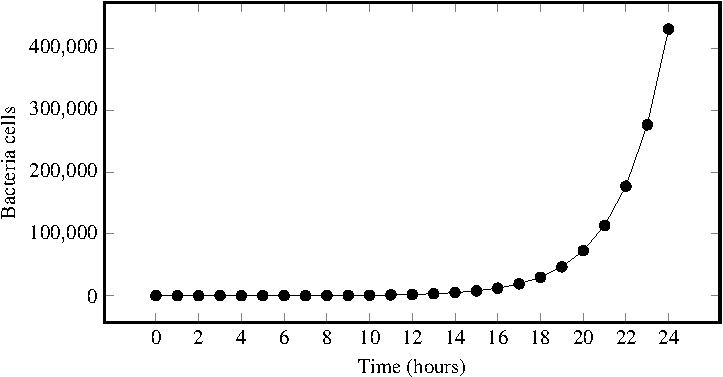
\includegraphics[scale=1.1]{image/11/bacteria.pdf}
\caption{%%
  The bacteria population in a Petri dish within $24$ hours.
  Initially, the Petri dish had a population of $10$ bacteria cells
  and the bacteria population is assumed to grow at a constant
  percentage rate of $56\%$ per hour.
}
\label{fig:bacteria_population_24_hours}
\end{figure}

\begin{exercise}
This is a continuation of \Example{eg:bacterial_growth}.
%%
\begin{packedenum}
\item\label{subex:bacteria_100_cells}
  How long must you wait for the bacteria population to be at least
  $100$ cells?

\item\label{subex:bacteria_doubling_time}
  Use the rule of $72$ to calculate a rough estimate of the doubling
  time of the bacteria population.  Use the growth formula of the
  bacteria population to verify your estimate and provide an upper
  bound on the doubling time.
\end{packedenum}
\end{exercise}

\ifbool{showSolution}{
\begin{solution}
\solutionpart{subex:bacteria_100_cells}
Using \Equation{eqn:bacterial_growth}, after $t = 5$ hours the
bacteria population would be approximately
\[
Q(5)
=
10 \times 1.56^5
\approx
92
\]
cells, rounded to the nearest integer.  After $t = 6$ hours, the
bacteria population would be approximately
\[
Q(6)
=
10 \times 1.56^6
\approx
144
\]
cells, rounded to the nearest integer.  Therefore you must wait at
most six hours in order for the bacteria population to be at least
$100$ cells.

\solutionpart{subex:bacteria_doubling_time}
You want to know the amount of time required for the bacteria
population to increase from the initial population of $10$ cells to
$20$ cells.  Since the bacteria population grows at a constant
percentage rate of $56\%$ per hour, the rule of $72$ states that the
doubling time of the population is approximately $72 / 56 = 1.2857$
hours, rounded to four decimal places.  Substituting this value into
\Equation{eqn:bacterial_growth} shows that after approximately
$1.2857$ hours the number of bacteria cells has increased to
\[
Q(1.2857)
=
10 \times 1.56^{1.2857}
\approx
17.7133
\]
cells, rounded to four decimal places.  This is below $20$ cells.  If
you substitute $t = 2$ hours into \Equation{eqn:bacterial_growth}, you
obtain
\[
Q(2)
=
10 \times 1.56^2
\approx
24.336.
\]
In other words, the doubling time of the bacteria population is
approximately $1.2857$ hours and at most $2$ hours.
\end{solution}
}{}

\begin{exercise}
\textbf{Population of Sweden.}
According to Statistiska centralbyr{\aa}n~(Statistics Sweden), by the
end of February 2018 the population of Sweden was approximately
$10.135303$ million people.\footnote{
  Data are from the following website:
  \url{https://web.archive.org/web/20180425041449/http://www.scb.se/BE0101-en},
  accessed 2018-04-25.
}
This is an increase of $1.2\%$ since the same period in 2017.  Assume
that the above figure is the population of Sweden in 2018.  Further
assume that for the next few years the population of Sweden will
increase by a constant percentage rate of $1.2\%$ per annum.
%%
\begin{packedenum}
\item\label{subex:Sweden_population_growth_rate_factor}
  Determine the constant growth rate and growth factor of the
  population of Sweden.

\item\label{subex:Sweden_population_2019_2020}
  Calculate the projected population of Sweden in the years 2019 and
  2020.

\item\label{subex:Sweden_population_formula_graph}
  Derive a formula for the population of Sweden after $t$ years since
  2018.  Use the formula to check your results
  from \Part{subex:Sweden_population_2019_2020}.  Produce a graph of
  the population of Sweden from the year 2018 up to and including
  2030.

\item\label{subex:Sweden_population_doubling_time}
  Use the rule of $72$ to calculate a rough estimate of the doubling
  time of the population of Sweden.  Verify your result with the
  formula from \Part{subex:Sweden_population_formula_graph} and use
  the formula to obtain an upper bound on the doubling time.
\end{packedenum}
\end{exercise}

\ifbool{showSolution}{
\begin{solution}
\solutionpart{subex:Sweden_population_growth_rate_factor}
The constant percentage growth rate is $1.2\%$.  Divide this number by
$100$ to get the constant growth rate of $r = 1.2 / 100 = 0.012$.
Then the growth factor is $b = 1 + 0.012 = 1.012$.

\solutionpart{subex:Sweden_population_2019_2020}
At time $t = 0$, the year is 2018 and the population is assumed to be
$10.135303$ million people.  At time $t = 1$, the year would be 2019
and the population would have increased by $10.135303 \times 0.012$
million people.  Add this number to the population at time $t = 0$ to
get
%%
\begin{align*}
&10.135303 + 10.135303 \times 0.012 \\[4pt]
&=
10.135303 (1 + 0.012) \\[4pt]
&=
10.135303 \times 1.012 \\[4pt]
&=
10.256926636
\end{align*}
%%
million people, which is the projected population of Sweden in 2019.
At time $t = 2$, the year would be 2020 and the population would have
increased by
\[
10.256926636 \times 0.012
\]
million people.  Add this number to the population at time $t = 1$ and
you obtain
%%
\begin{align*}
&10.256926636 + 10.256926636 \times 0.012 \\[4pt]
&=
10.256926636 (1 + 0.012) \\[4pt]
&=
10.256926636 \times 1.012 \\[4pt]
&=
10.380009755632
\end{align*}
%%
million people, which is the projected population of Sweden in 2020.

\begin{figure}[!htbp]
\centering
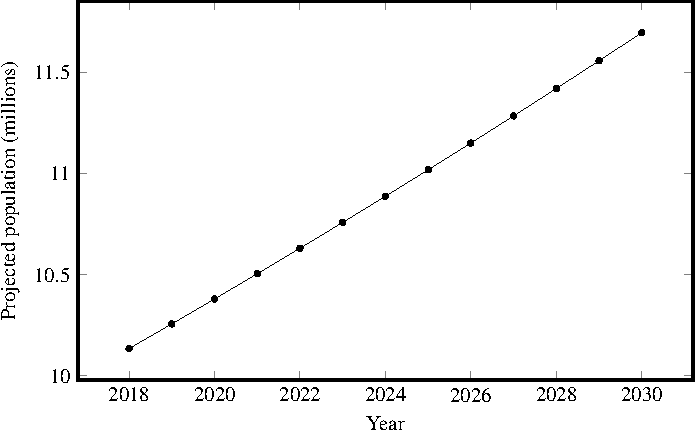
\includegraphics[scale=1.1]{image/11/population-sweden.pdf}
\caption{%%
  The projected population of Sweden from the year 2018 up to and
  including 2030.  It is assumed that the population of Sweden in 2018
  is $10.135303$ million people and that the population increases by a
  constant percentage rate of $1.2\%$ per annum.
}
\label{fig:population_Sweden}
\end{figure}

\solutionpart{subex:Sweden_population_formula_graph}
You assume that the population of $a = 10.135303$ million people in
2018 is the initial population.
From \Part{subex:Sweden_population_growth_rate_factor} you know that
the growth factor is $b = 1.012$.  If $Q(t)$ represents the
population~(in millions) of Sweden in $t$ years since 2018, use
\Theorem{thm:exponential_growth} to write
%%
\begin{equation}
\label{eqn:Sweden_population_formula}
Q(t)
=
10.135303 \times 1.012^t.
\end{equation}
%%
Using the latter formula, at $t = 1$ year since 2018 the population of
Sweden is projected to be
\[
Q(1)
=
10.135303 \times 1.012^1
=
10.256926636
\]
million people.  At $t = 2$ years since 2018, the projected population
of Sweden is
\[
Q(2)
=
10.135303 \times 1.012^2
=
10.380009755632
\]
million people.  These numbers are consistent with the results
in \Part{subex:Sweden_population_2019_2020}.
\Figure{fig:population_Sweden} shows a graph of the projected
population of Sweden from 2018 up to and including the year 2030.

\solutionpart{subex:Sweden_population_doubling_time}
You want to determine the amount of time~(in years) required for the
population of Sweden to increase from $10.135303$ million people to
$10.135303 \times 2 = 20.270606$ million people.  Since the population
is assumed to grow at a constant percentage rate of $1.2\%$ per annum,
the rule of $72$ yields a doubling time of approximately
$72 / 1.2 = 60$ years.  Substituting the value of $t = 60$ into
\Equation{eqn:Sweden_population_formula} shows that after $60$ years
since $2018$ the population of Sweden would have increased to
approximately
\[
Q(60)
=
10.135303 \times 1.012^{60}
\approx
20.7332548929601
\]
million people, which is higher than the required number of
$20.270606$ million people.  However, if you substitute $t = 59$ into
\Equation{eqn:Sweden_population_formula} you get
\[
Q(59)
=
10.135303 \times 1.012^{59}
\approx
20.4874060207115
\]
and substituting $t = 58$ into
\Equation{eqn:Sweden_population_formula} again shows that
\[
Q(58)
=
10.135303 \times 1.012^{58}
\approx
20.2444723524818.
\]
Therefore the required doubling time is approximately $60$ years and
at most $59$ years.
\end{solution}
}{}

\begin{exercise}
\textbf{E. coli.}
A variant of \emph{E.~coli} called \emph{E.~coli O157:H7} is a type of
bacteria that cause food poisoning.\footnote{
  See the following paper for further details:
  \url{https://www.ncbi.nlm.nih.gov/pmc/articles/PMC3645889/}.
}
At a temperature of $\degree{37}$C, \emph{E.~coli O157:H7} has a
doubling time of approximately $24$ minutes.\footnote{
  According to the following fact sheet:
  \url{http://web.archive.org/web/20180425054209/http://www.foodsafety.govt.nz/elibrary/industry/Escherichia_Coli-Organism_Invades.pdf},
  accessed 2018-04-27.
}
Suppose a piece of raw meat contains five cells of
\emph{E.~coli O157:H7}.
%%
\begin{packedenum}
\item\label{subex:E_coli_formula_graph}
  Use the doubling time above to derive a formula for the growth of
  the \emph{E.~coli} population.  Produce a graph of the bacteria
  population up to $4.8$ hours.

\item\label{subex:E_coli_1000_cells}
  Calculate the amount of time~(in hours) required for the
  \emph{E.~coli} population to exceed $1000$ cells.
\end{packedenum}
\end{exercise}

\ifbool{showSolution}{
\begin{solution}
\solutionpart{subex:E_coli_formula_graph}
The doubling time is $24$ minutes, which means that a population of
\emph{E.~coli} O157:H7 will increase by $100\%$ every $24$ minutes.
The constant rate of growth is $r = 100 / 100 = 1$ and the growth
factor is $b = 1 + 1 = 2$.  The initial population is $a = 5$ cells.
Let $t$ be the number of doublings.  Use
\Theorem{thm:exponential_growth} to write the population $Q(t)$ after
$t$ doublings as
%%
\begin{equation}
\label{eqn:ecoli_growth}
Q(t)
=
5 \times 2^t.
\end{equation}
%%
The time frame of $4.8$ hours is equivalent to $4.8 \times 60 = 288$
minutes.  Divide this number by $24$ to get $288 / 24 = 12$, which
means that within a time span of $4.8$ hours the bacteria population
would have undergone $12$ doublings.  \Figure{fig:ecoli_growth} shows
a graph of the growth of the \emph{E.~coli} population.

\begin{figure}[!htbp]
\centering
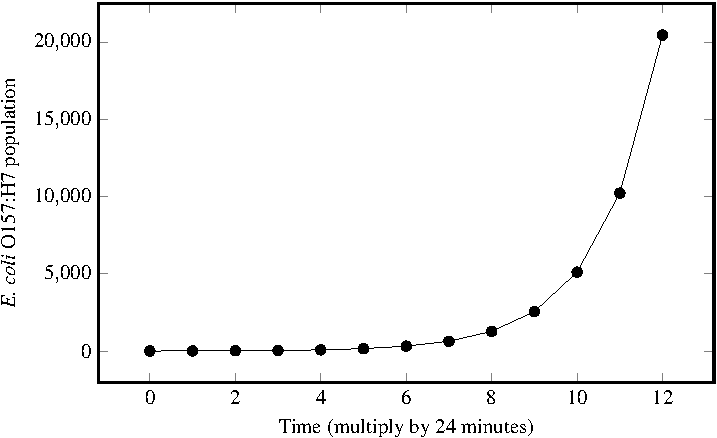
\includegraphics[scale=1.1]{image/11/ecoli.pdf}
\caption{%%
  The growth of an \emph{E.~coli} O157:H7 population within the span
  of $4.8$ hours.  The initial population is five cells and the
  doubling time is $24$ minutes.  The horizontal axis shows the number
  of doublings.  Multiply the number of doublings $t$ by $24$ to
  obtain $24t$ minutes.
}
\label{fig:ecoli_growth}
\end{figure}

\solutionpart{subex:E_coli_1000_cells}
Substitute $t = 7$ into \Equation{eqn:ecoli_growth} and you get
\[
Q(7)
=
5 \times 2^7
=
640
\]
cells.  Perform the same substitution with $t = 8$ and you get
\[
Q(8)
=
5 \times 2^8
=
1280
\]
cells.  At $t = 8$ doublings, the elapsed time would be
$8 \times 24 = 192$ minutes, which is equivalent to
$192 / 60 = 3.2$ hours.  In other words, you must wait at most $3.2$
hours for the \emph{E.~coli} population to exceed $1000$ cells.
\end{solution}
}{}


%%%%%%%%%%%%%%%%%%%%%%%%%%%%%%%%%%%%%%%%%%%%%%%%%%%%%%%%%%%%%%%%%%%%%%%%%%%

\section{Exponential decay}

When a population or the amount of something decreases exponentially,
instead of a constant growth rate you now have a constant
\emph{decay rate} $r$.  Multiply $r$ by $100\%$ to get the constant
percentage rate of decay.  Furthermore, instead of a growth factor you
now have a constant \emph{decay factor} $b$.  The constant decay
factor is defined as one minus the decay rate so $b = 1 - r$.  You can
think of the decay factor as the fraction of something remaining after
unit time.  For instance, if the amount of water in a bucket decreases
by a constant percentage rate of $5.6\%$ per minute, the constant
decay rate is $5.6 / 100 = 0.056$ per minute.  The constant decay
factor would be $1 - 0.056 = 0.944$.  Multiply this number by $100\%$
to get $0.944 \times 100\% = 94.4\%$.  In other words, each minute the
bucket loses $5.6\%$ of the amount of water it holds, but the bucket
still has $94.4\%$ of the amount of water.  If $a$ is the initial
population and $Q(t)$ represents the population at time $t$, then
$Q(t)$ can be written as
%%
\begin{equation}
\label{eqn:exponential_decay}
Q(t)
=
ab^t.
\end{equation}
%%
You can derive \Equation{eqn:exponential_decay} by using the same
reasoning that led to \Equation{eqn:exponential_growth}.  Note that
\Equation{eqn:exponential_decay} is almost identical to the equation
for exponential growth in \Theorem{thm:exponential_growth}.  The above
discussion is summarised in \Theorem{thm:exponential_decay}.
\Figure{fig:exponential_decay} shows a graph of what an exponential
decay looks like.

\begin{figure}[!htbp]
\centering
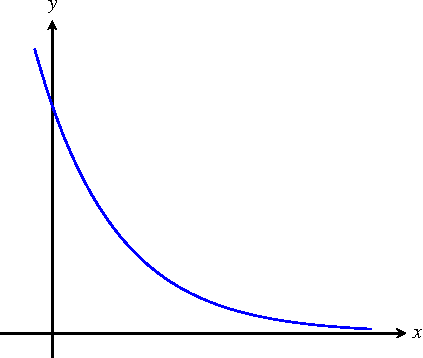
\includegraphics[scale=1.1]{image/11/exponential-decay.pdf}
\caption{%%
  A general graph of exponential decay.
}
\label{fig:exponential_decay}
\end{figure}

\begin{theorem}
\label{thm:exponential_decay}
\textbf{Exponential decay.}
Let $a \neq 0$ be the initial value of a population.  Assume that the
population decreases by a constant decimal rate of $r$ per unit time.
If $b = 1 - r$ is the decay factor and $Q(t)$ represents the
population number at time $t$, then $Q(t) = ab^t$.
\end{theorem}

Just as an exponential growth has a doubling time, an exponential
decay has a \emph{half-life}.  The half-life of an exponential decay
is the amount of time required to reach $50\%$ of the initial
quantity.  For instance, refer to the bucket example above.  Suppose a
bucket holds three litres of water.  At the bottom of the bucket is a
hole, out of which water leaks at a constant percentage rate of
$5.6\%$ per minute.  To understand the half-life of this exponential
decay model, you ask the question:  How long must you wait for the
amount of water in the bucket to decrease to $50\%$ of the original
quantity?  That is, how long would it require for the amount of water
in the bucket to decrease to $3 / 2 = 1.5$ litres?  You can use the
formula that models the amount of water in the bucket to estimate the
half-life of the model.  Or you can use the \emph{rule of 69} to
calculate an approximation of the half-life.

The rule of $69$ is a way to obtain a rough estimate of the half-life
of an exponential decay model.  Let $a$ be the initial population or
quantity.  If $r$ is the constant decay rate as a decimal, then
$p = r \times 100\%$ is the constant decay rate as a percentage.
According to the rule of $69$, the half-life of the decay model can be
approximated as $69 / p$.  If you know a formula for the exponential
decay, you can use the formula together with the rule of $69$ in order
to calculate a better estimate of the half-life.
\Example{eg:water_level} clarifies this point and the rule of $69$ is
summarised in \Theorem{thm:rule_of_69}.

\begin{theorem}
\label{thm:rule_of_69}
\textbf{Rule of $69$.}
In an exponential decay model, let $p$ be the constant decay rate as a
percentage.  The half-life of the model is approximately $69 / p$
units of time.
\end{theorem}

\begin{figure}[!htbp]
\centering
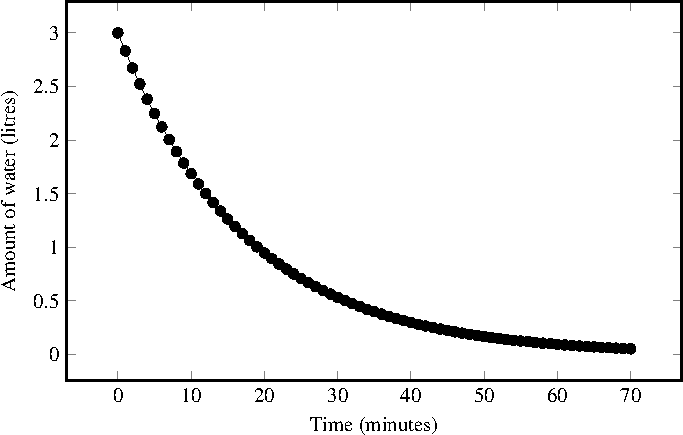
\includegraphics[scale=1.1]{image/11/water.pdf}
\caption{%%
  The amount~(in litres) of water remaining in a bucket after $t$
  minutes.  The bucket has an initial quantity of three litres of
  water and water leaks out of the bucket at a constant percentage
  rate of $5.6\%$ per minute.
}
\label{fig:bucket_water_level}
\end{figure}

\begin{example}
\label{eg:water_level}
\textbf{Water level.}
A bucket contains three litres of water.  Water leaks out of the
bucket at a constant percentage rate of $5.6\%$ per minute.
%%
\begin{packedenum}
\item\label{subex:water_level_formula}
  Derive a formula that models the amount~(in litres) of water in the
  bucket after $t$ minutes.  Use the formula to produce a graph of the
  amount of water in the bucket up to $t = 70$ minutes.

\item\label{subex:water_level_half_life}
  Estimate the half-life of the exponential decay model.
\end{packedenum}
\end{example}

\begin{solution}
\solutionpart{subex:water_level_formula}
The initial amount of water is $a = 3$ litres.  The constant decay
rate is $r = 5.6 / 100 = 0.056$ per minute, thus the decay factor is
$b = 1 - 0.056 = 0.944$.  If $W(t)$ represents the amount~(in litres)
of water in the bucket after $t$ minutes, use
\Theorem{thm:exponential_decay} to write
%%
\begin{equation}
\label{eqn:bucket_water_level}
W(t)
=
3 \times 0.944^t.
\end{equation}
%%
See \Figure{fig:bucket_water_level} for a graph of the amount of water
in the bucket up to $70$ minutes.

\solutionpart{subex:water_level_half_life}
The half-life of the exponential model~\eqref{eqn:bucket_water_level}
is the amount of time~(in minutes) required for the quantity of water
in the bucket to decrease to $50\%$ of the original amount.  The
bucket originally has three litres of water.  You want to know how
long you must wait for the quantity of water in the bucket to decrease
to $3 / 2 = 1.5$ litres.  Substituting $t = 12$ into
\Equation{eqn:bucket_water_level} yields
\[
W(12)
=
3 \times 0.944^{12}
\approx
1.5024
\]
litres, rounded to four decimal places.  Furthermore, substitute
$t = 13$ into \Equation{eqn:bucket_water_level} and you get
\[
W(13)
=
3 \times 0.944^{13}
\approx
1.4183
\]
litres, also rounded to four decimal places.  Therefore the half-life
of the model~\eqref{eqn:bucket_water_level} is approximately $12$
minutes.
\end{solution}

\begin{example}
\label{eg:radiocarbon_dating}
\textbf{Radiocarbon dating.}
The amount of carbon-$14$ found in a fossil~(e.g.~an ancient bone or
wood) can be used to determine the age of the fossil.  Assume that the
amount of carbon-$14$ decreases by a constant percentage rate of
approximately $11.4\%$ every $1000$ years.\footnote{
  The most accurate estimation is that the amount of carbon-$14$ in a
  fossil decreases by $50\%$ approximately every $5,730$ years.  See
  the following paper for further details:
  \url{http://doi.org/10.1038/195984a0}.  Where did the $11.4\%$ come
  from?  After $1000$ years, the initial amount of $300$ micrograms of
  carbon-$14$ would have decreased to approximately $265.818669$
  micrograms, rounded to six decimal places.  The fraction of
  carbon-$14$ remaining is the ratio $265.818669 / 300$ and therefore
  the initial amount would have decreased by a fraction of
  \[
  1 - \frac{265.818669}{300}
  =
  0.11393777.
  \]
  Multiply the result by $100\%$ to get $11.393777\%$, which can be
  rounded to $11.4\%$.  See the following video for an explanation of
  carbon-14 dating: \url{https://youtu.be/phZeE7Att_s}.  The next
  video explains the process of radioactive decay:
  \url{https://youtu.be/oFdR_yMKOCw}.
}
Suppose that you start with $300$ micrograms of carbon-$14$.
%%
\begin{packedenum}
\item\label{subeg:carbon14_decay_rate}
  Determine the constant decay rate.  Provide an interpretation of
  this rate.

\item\label{subeg:carbon14_decay_factor}
  Calculate the decay factor.  Provide an interpretation of the decay
  factor.

\item\label{subeg:carbon14_after_1000_and_2000_years}
  Determine the amount of carbon-$14$ remaining after $1000$ years and
  after $2000$ years.

\item\label{subeg:carbon14_formula_graph}
  Derive a formula for the amount of carbon-$14$ remaining.  Produce a
  graph of the amount of carbon-$14$ remaining up to and including the
  first $50,000$ years.
\end{packedenum}
\end{example}

\begin{solution}
\solutionpart{subeg:carbon14_decay_rate}
The constant percentage rate of decay is $11.4\%$ every $1000$ years.
Divide the number $11.4$ by $100$ to get the constant decay rate of
$r = 11.4 / 100 = 0.114$ per $1000$ years.  The decay rate of $0.114$
tells you that you lose $11.4\%$ of the amount of carbon-$14$ every
$1000$ years.

\solutionpart{subeg:carbon14_decay_factor}
The decay factor is $b = 1 - 0.114 = 0.886$, which can be converted to
a percentage as $0.886 \times 100 = 88.6\%$.  In other words, after
every $1000$ years you lose $11.4\%$ of the amount of carbon-$14$ or
that only about $88.6\%$ of the amount of carbon-$14$ remains.  You
might lose $11.4\%$ of the amount, but you still have $88.6\%$ left.

\solutionpart{subeg:carbon14_after_1000_and_2000_years}
After $1000$ years, you would have lost $300 \times 0.114$ micrograms
of carbon-$14$.  Subtract this number from the original amount to get
%%
\begin{align*}
300 - 300 \times 0.114
&=
300 (1 - 0.114) \\[4pt]
&=
300 \times 0.886 \\[4pt]
&=
265.8.
\end{align*}
%%
That is, after $1000$ years you would have $265.8$ micrograms of
carbon-$14$ left.  At the end of $2000$ years, you would have lost
$265.8 \times 0.114$ micrograms of carbon-$14$.  Subtract this amount
from $265.8$ to get
%%
\begin{align*}
265.8 - 265.8 \times 0.114
&=
265.8 (1 - 0.114) \\[4pt]
&=
265.8 \times 0.886 \\[4pt]
&=
235.4988.
\end{align*}
%%
In other words, after $2000$ years you would have only $235.4988$
micrograms of carbon-$14$ left.

\solutionpart{subeg:carbon14_formula_graph}
The unit of time $t$ is $1000$ years.  An increase of $t$ by one unit
translates to an increase by $1000$ years.  You have an initial amount
of $300$ micrograms of carbon-$14$ and a decay factor of $0.886$.  If
$A(t)$ represents the amount of carbon-$14$ remaining at time $t$, use
\Theorem{thm:exponential_decay} to write $A(t) = 300 \times 0.886^t$.
Note that $t$ is in terms of $1000$ years.  So $t = 1$ means
$1 \times 1000 = 1000$ years, $t = 2$ means $2 \times 1000 = 2000$
years, $t = 3$ means $3 \times 1000 = 3000$ years, and so on.

To produce a graph of the amount of carbon-$14$ left after $50,000$
years, you must work out the minimum and maximum values for $t$.  The
value of $t = 0$ means the time at which you have the initial amount
of carbon-$14$ so you take $t = 0$ as the minimum value.  Since $t$ is
in terms of $1000$ years, divide $50,000$ by $1000$ to get
$t = 50000 / 1000 = 50$ so that the maximum value of $t$ is
$t = 50$.  \Figure{fig:carbon14_decay} shows a graph of the amount of
carbon-$14$ remaining up to $50,000$ years later.
\end{solution}

\begin{figure}[!htbp]
\centering
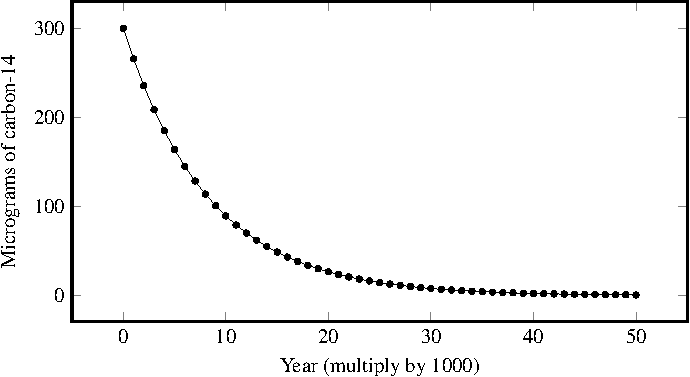
\includegraphics[scale=1.1]{image/11/carbon14.pdf}
\caption{%%
  The amount~(in micrograms) of carbon-$14$ remainining after
  $t \times 1000$ years.  You initially have $300$ micrograms of
  carbon-$14$.  It is assumed that the constant percentage decay
  rate of carbon-$14$ is $11.4\%$ per $1000$ years.
}
\label{fig:carbon14_decay}
\end{figure}

\begin{exercise}
Use the formula from the solution of
\Subexample{eg:radiocarbon_dating}{subeg:carbon14_formula_graph} to
verify the solution in
\Subexample{eg:radiocarbon_dating}{subeg:carbon14_after_1000_and_2000_years}.
\end{exercise}

\ifbool{showSolution}{
\begin{solution}
Suppose the initial amount of carbon-$14$ is $300$ micrograms and that
carbon-$14$ decreases at a constant percentage rate of $11.4\%$ per
$1000$ years.  From
\Subexample{eg:radiocarbon_dating}{subeg:carbon14_formula_graph}, the
amount $A(t)$ in micrograms of carbon-$14$ remaining after
$t \times 1000$ years can be written as $A(t) = 300 \times 0.886^t$.
After $1000$ years, you have $t = 1$ and substitute $t = 1$ into the
formula to get
\[
A(1)
=
300 \times 0.886^1
=
265.8
\]
micrograms.  After $2000$ years, you have $t = 2$.  Substitute
$t = 2$ into the formula to get
\[
A(2)
=
300 \times 0.886^2
=
235.4988
\]
micrograms.  These numbers are the same as those obtained in the
solution of
\Subexample{eg:radiocarbon_dating}{subeg:carbon14_after_1000_and_2000_years}.
\end{solution}
}{}

\begin{exercise}
\textbf{Radioactive decay of fermium-$250$.}
The isotope known as fermium-$250$ has a half-life of $30$
minutes.\footnote{
  See the following paper for the original discovery:
  \url{https://doi.org/10.1103/PhysRev.95.585.2}.  The next video
  explains the half-life of radioactive decay in terms of rolling
  dice:
  \url{https://youtu.be/HRwey6cwGHo}.
}
That is, a given amount of fermium-$250$ will decrease by $50\%$ every
$30$ minutes.  Suppose you start with $100$ micrograms of
fermium-$250$.
%%
\begin{packedenum}
\item\label{subex:fermium250_decay_rate}
  Determine the constant decay rate.  Provide an interpretation of
  this rate.

\item\label{subex:fermium250_decay_factor}
  Calculate the decay factor.  Provide an interpretation of this
  factor.

\item\label{subex:fermium250_30minutes_60minutes}
  Calculate the amount of fermium-$250$ remaining after $30$ minutes
  and after an hour.

\item\label{subex:fermium250_decay_formula}
  Derive a formula for the amount of fermium-$250$ remaining.  Use the
  formula to verify your results
  from \Part{subex:fermium250_30minutes_60minutes}.  Produce a graph
  of the amount of fermium-$250$ remaining up to and including $12$
  hours.

\item\label{subex:fermium250_less_than_1microgram}
  How long must you wait for the amount of fermium-$250$ to be less
  than one microgram?
\end{packedenum}
\end{exercise}

\ifbool{showSolution}{
\begin{solution}
\solutionpart{subex:fermium250_decay_rate}
Since the constant percentage decay rate is $50\%$, the constant decay
rate is $r = 50 / 100 = 0.5$.  This means that after each $30$ minutes
the amount of fermium-$250$ decreases by a rate of $0.5$.

\solutionpart{subex:fermium250_decay_factor}
The decay factor is defined as one minus the decay rate so
$b = 1 - 0.5 = 0.5$.  Multiply this number by $100\%$ to get
$0.5 \times 100\% = 50\%$.  After each $30$ minutes only $50\%$ of the
amount of fermium-$250$ remains.

\solutionpart{subex:fermium250_30minutes_60minutes}
The unit of time $t$ is $30$ minutes.  An increase of $t$ by one unit
means that time would have increased by $30$ minutes.  You start with
$100$ micrograms of fermium-$250$ at time $t = 0$.  At time $t = 1$ or
after $30$ minutes, the amount of fermium-$250$ would have decreased
by $100 \times 0.5$ micrograms.  Subtract this number from the amount
at time $t = 0$ to get
%%
\begin{align*}
100 - 100 \times 0.5
&=
100 (1 - 0.5) \\[4pt]
&=
100 \times 0.5 \\[4pt]
&=
50
\end{align*}
%%
micrograms of fermium-$250$.  At time $t = 2$ or after an hour, the
amount of fermium-$250$ would have decreased by $50 \times 0.5$
micrograms.  Subtract this number from the amount at time $t = 1$ to
get
%%
\begin{align*}
50 - 50 \times 0.5
&=
50 (1 - 0.5) \\[4pt]
&=
50 \times 0.5 \\[4pt]
&=
25
\end{align*}
%%
micrograms of fermium-$250$.

\begin{figure}[!htbp]
\centering
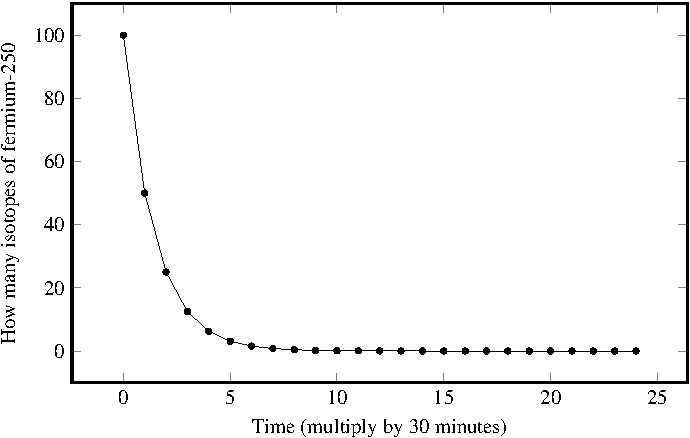
\includegraphics[scale=1.1]{image/11/fermium250.pdf}
\caption{%%
  A graph of the amount~(in micrograms) of the isotope fermium-$250$
  after every $30$ minutes.  The unit of time $t$ is $30$ minutes so
  multiply each number on the horizontal axis by $30$ to get the
  number of minutes.  Here you start with $100$ micrograms of
  fermium-$250$.  The isotope is known to decay at a constant
  percentage rate of $50\%$ every $30$ minutes.
}
\label{fig:fermium250_decay}
\end{figure}

\solutionpart{subex:fermium250_decay_formula}
You know that the initial amount of fermium-$250$ is $a = 100$
micrograms and that the decay factor is $b = 0.5$.  Let each unit of
time $t$ be $30$ minutes.  If $A(t)$ represents the amount of
fermium-$250$ remaining after $t$ units of time, use
\Theorem{thm:exponential_decay} to write $A(t) = 100 \times 0.5^t$.
Let's use the latter formula to verify the results
from \Part{subex:fermium250_30minutes_60minutes}.  The time of
$t = 1$ translates to $30$ minutes so at time $t = 1$ you would have
\[
A(1)
=
100 \times 0.5^1
=
50
\]
micrograms of fermium-$250$.  The time of $t = 2$ translates to
$2 \times 30 = 60$ minutes so at time $t = 2$ you would have
\[
A(2)
=
100 \times 0.5^2
=
25
\]
micrograms of fermium-$250$.  These are the same numbers as those
obtained in \Part{subex:fermium250_30minutes_60minutes}.
\Figure{fig:fermium250_decay} shows a graph of the decrease in the
amount of fermium-$250$ after every $30$ minutes.

\solutionpart{subex:fermium250_less_than_1microgram}
At time $t = 6$, the elapsed time would be $6 \times 30 = 180$ minutes
and the amount of fermium-$250$ remaining is
\[
A(6)
=
100 \times 0.5^6
=
1.5625
\]
micrograms.  At time $t = 7$, the elapsed time would be
$7 \times 30 = 210$ minutes and the amount of fermium-$250$ remaining
is
\[
A(7)
=
100 \times 0.5^7
=
0.78125
\]
micrograms.  Divide $210$ by $60$ minutes to get $3.5$ hours.
Therefore you must wait approximately $3.5$ hours in order for the
amount of fermium-$250$ to be less than one microgram.
\end{solution}
}{}

\begin{exercise}
\textbf{Newton's law of cooling.}
A pot of soup has a temperature of $100$ degrees Celsius.  The
temperature of the pot decreases at a constant percentage rate of
approximately $1.8\%$ per minute.
%%
\begin{packedenum}
\item\label{subex:soup_temperature_1minute_2minutes}
  Calculate the temperature of the pot of soup after one minute.  Do
  the same for after two minutes.

\item\label{subex:soup_temperature_formula_graph}
  Derive a formula for the temperature of the pot of soup after $t$
  minutes.  Use the formula to verify your results
  from \Part{subex:soup_temperature_1minute_2minutes}.  Produce a
  graph of the temperature of the pot of soup up to after three
  hours.

\item\label{subex:soup_temperature_half_life}
  Estimate the half-life of the temperature of the pot of soup.

\item\label{subex:soup_temperature_15_degrees}
  How long must you wait for the temperature of the pot of soup to be
  less than $15$ degrees Celsius?
\end{packedenum}
\end{exercise}

\ifbool{showSolution}{
\begin{solution}
\solutionpart{subex:soup_temperature_1minute_2minutes}
The initial temperature of the pot of soup is $a = 100$ degrees
Celsius.  The constant percentage rate of cooling is $1.8\%$ and so
the constant rate at which the temperature of the pot of soup
decreases is $r = 0.018$.  After one minute, the temperature of the
pot would have decreased by $100 \times 0.018$ degrees Celsius.
Subtract this number from the initial temperature to get
%%
\begin{align*}
100 - 100 \times 0.018
&=
100 (1 - 0.018) \\[4pt]
&=
100 \times 0.982 \\[4pt]
&=
98.2
\end{align*}
%%
degrees Celsius.  At time $t = 2$ minutes, the temperature of the pot
would have decreased by $98.2 \times 0.018$ degrees Celsius.  Subtract
this number from the temperature at time $t = 1$ minute to get
%%
\begin{align*}
98.2 - 98.2 \times 0.018
&=
98.2 (1 - 0.018) \\[4pt]
&=
98.2 \times 0.982 \\[4pt]
&=
96.4324
\end{align*}
%%
degrees Celsius.

\solutionpart{subex:soup_temperature_formula_graph}
From \Part{subex:soup_temperature_1minute_2minutes} you know that the
initial temperature of the pot of soup is $a = 100$ degrees Celsius
and the constant rate of cooling is $r = 0.018$.  Then the cooling
factor~(i.e.~the decay factor) is $b = 1 - 0.018 = 0.982$.  If $T(t)$
represents the temperature~(in degrees Celsius) of the pot of soup
after $t$ minutes, use \Theorem{thm:exponential_decay} to write
%%
\begin{equation}
\label{eqn:soup_temperature}
T(t)
=
100 \times 0.982^t.
\end{equation}
%%
Using the latter formula, after $t = 1$ minute the temperature of the
pot would be
\[
T(1)
=
100 \times 0.982^1
=
98.2
\]
degrees Celsius.  After $t = 2$ minutes, the temperature of the pot
would be
\[
T(2)
=
100 \times 0.982^2
=
96.4324
\]
degrees Celsius.  These numbers are the same as those obtained
in \Part{subex:soup_temperature_1minute_2minutes}.
\Figure{fig:soup_temperature} shows a graph of the temperature of the
pot of soup up to after $180$ minutes or three hours.

\begin{figure}[!htbp]
\centering
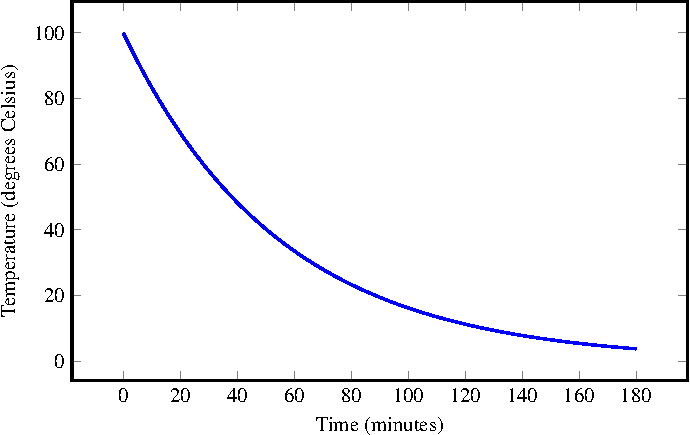
\includegraphics[scale=1.1]{image/11/soup.pdf}
\caption{%%
  The temperature~(in degrees Celsius) of a pot of soup after $t$
  minutes.  The pot has an initial temperature of $100$ degrees
  Celsius.  The temperature decreases at a constant percentage rate of
  approximately $1.8\%$ per minute.
}
\label{fig:soup_temperature}
\end{figure}

\solutionpart{subex:soup_temperature_half_life}
You want to determine the amount of time required for the temperature
of the pot of soup to be $50\%$ of its original temperature.  That is,
you want to know how long you must wait for the temperatore of the pot
to be $100 / 2 = 50$ degrees Celsius.  The graph in
\Figure{fig:soup_temperature} shows that after approximately $40$
minutes, the temperature of the pot would be roughly $50$ degrees
Celsius.  Substituting $t = 40$ into \Equation{eqn:soup_temperature}
produces
\[
T(40)
=
100 \times 0.982^{40}
\approx
48.36
\]
degrees Celsius, rounded to two decimal places.  In fact, substituting
$t = 38$ into \Equation{eqn:soup_temperature} results in
\[
T(38)
=
100 \times 0.982^{38}
\approx
50.15
\]
degrees Celsius, also rounded to two decimal places.  You can conclude
that the half-life of the temperature of pot is approximately $38$
minutes.

\solutionpart{subex:soup_temperature_15_degrees}
After $t = 104$ minutes, the temperature of the pot of soup would be
approximately
\[
T(104)
=
100 \times 0.982^{104}
\approx
15.12
\]
degrees Celsius, rounded to two decimal places.  After $t = 105$
minutes, the temperature would be approximately
\[
T(105)
=
100 \times 0.982^{105}
\approx
14.85
\]
degrees Celsius, rounded to two decimal places.  Therefore you must
wait approximately $105$ minutes or approximately
$105 / 60 = 1.75$ hours in order for the temperature of the pot of
soup to be less than $15$ degrees Celsius.
\end{solution}
}{}

\begin{exercise}
An M\&M's experiment to understand half-life.
\end{exercise}

\ifbool{showSolution}{
\begin{solution}

\end{solution}
}{}


%%%%%%%%%%%%%%%%%%%%%%%%%%%%%%%%%%%%%%%%%%%%%%%%%%%%%%%%%%%%%%%%%%%%%%%%%%%

\section{Compound interest}

The \emph{interest} on a given amount of money is the additional
amount on top of the given amount.  When you deposit money into a
savings account, interest is usually calculated on your account
balance and then added to your balance.  The more money your savings
account has and the longer you leave the account open, the more
interest you would earn.  In the context of a savings account, you
would like the interest rate to be as high as possible and the time
between interest calculations to be as short as possible.  When you
take out a loan, interest is calculated on the amount you still have
to repay.  In this case, you want the interest rate to be as low as
possible and the time between interest calculations to be as long as
possible.  \Example{eg:savings_6months} below should help you to
understand compound interest.\footnote{
  See the following video for an explanation of compound interest:
  \url{https://youtu.be/MhvjCWfy-lw}.
}

\begin{example}
\label{eg:savings_6months}
\textbf{Half-yearly compounding.}
At the start of a new year, you open a savings account and deposit
$\$100$ into the account.  The account earns an interest of $3\%$ per
annum, where interest is calculated every six months~(i.e.~the
compounding period is half-yearly).  Assume that once you have
deposited the $\$100$, you leave the account alone to accrue interest
and no longer deposit any more money into the account.
%%
\begin{packedenum}
\item\label{subeg:savings_6months_initial_balance}
  Determine the initial balance of your account.

\item\label{subeg:savings_6months_growth_rate}
  Determine the half-yearly interest rate.  Use this value to
  calculate the half-yearly growth rate and the half-yearly growth
  factor of your account balance.

\item\label{subeg:savings_6months_balance_first_year}
  Use the same technique as in
  \Expression{eqn:Australian_population_2018_calculation} to calculate
  the balance of your account at the end of the first six months.
  Calculate the balance of your account at the end of the first year.

\item\label{subeg:savings_6months_balance_formula}
  Derive a formula for your account balance after $t$ compounding
  periods.  Use the formula to verify your results
  from \Part{subeg:savings_6months_balance_first_year}.  Produce a
  graph of your account balance within the first three years since you
  opened the account.

\item\label{subeg:savings_6months_doubling_time}
  Estimate the doubling time of the balance of your account .
\end{packedenum}
\end{example}

\begin{solution}
\solutionpart{subeg:savings_6months_initial_balance}
Your account has an initial balance of $\$100$.

\solutionpart{subeg:savings_6months_growth_rate}
The annual interest rate is $3\%$.  However, interest is calculated
every six months.  That is, interest is compounded twice a year.
Divide $3$ by the number of compounding periods per year to get
$3 / 2 = 1.5$.  In other words, the half-yearly interest rate is
$1.5\%$.  The half-yearly growth rate is $r = 0.015$, hence the
half-yearly growth factor is $b = 1 + 0.015 = 1.015$.

\solutionpart{subeg:savings_6months_balance_first_year}
At the end of the first six months~(i.e.~$t = 1$, the time of the
first compounding), you would have earned an interest of
$100 \times 0.015$ dollars.  Add this amount to the initial balance to
get
%%
\begin{align*}
100 + 100 \times 0.015
&=
100 (1 + 0.015) \\[4pt]
&=
100 \times 1.015 \\[4pt]
&=
101.5.
\end{align*}
%%
After the first six months, your account balance would be
$\$101.50$.  At the end of the first year~(i.e.~$t = 2$, the time of
the second compounding), you would earn $101.5 \times 0.015$ dollars
in interest.  Add this amount to the balance at time $t = 1$ and you
have
%%
\begin{align*}
101.5 + 101.5 \times 0.015
&=
101.5 (1 + 0.015) \\[4pt]
&=
101.5 \times 1.015 \\[4pt]
&=
103.0225.
\end{align*}
%%
At the end of the first year, your account balance would be
approximately $\$103.02$, rounded to the nearest cent.

\solutionpart{subeg:savings_6months_balance_formula}
Let $t$ be the number of compounding periods, i.e.~the number of times
interest has been calculated.  Since interest is calculated every six
months, multiply $t$ by $6$ to see that when interest has been
compounded $t$ times then $6t$ months would have elapsed.  The initial
balance is $a = 100$ dollars and the constant growth factor is
$b = 1.015$.  If $B(t)$ represents the balance of your account when
interest has been compounded $t$ times, use
\Theorem{thm:exponential_growth} to write
%%
\begin{equation}
\label{eqn:compound_interest_a100_b1.015}
B(t)
=
100 \times 1.015^t.
\end{equation}
%%
The time of $t = 1$ corresponds to the end of the first six months.
Substitute $t = 1$ into \Equation{eqn:compound_interest_a100_b1.015}
to see that at the end of the first six months your account balance
would be
\[
B(1)
=
100 \times 1.015^1
=
101.5
\]
dollars.  The time of $t = 2$ corresponds to the end of the first
year.  Substituting $t = 2$ into
\Equation{eqn:compound_interest_a100_b1.015} shows that at the end of
the first year your account balance would be
\[
B(2)
=
100 \times 1.015^2
=
103.0225
\]
dollars.  These balance amounts are consistent with the results
from \Part{subeg:savings_6months_balance_first_year}.
\Figure{fig:compound_interest_a100_b1.015} shows a graph of the
account balance over a period of three years.

\begin{figure}[!htbp]
\centering
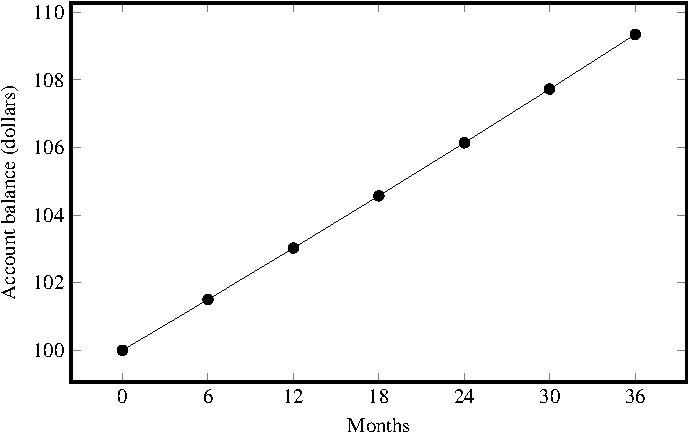
\includegraphics[scale=1.1]{image/11/interest-half-yearly.pdf}
\caption{%%
  The balance of a savings account over a period of three years.  The
  initial balance is $\$100$ with an interest rate of $3\%$ per annum,
  compounded every six months.
}
\label{fig:compound_interest_a100_b1.015}
\end{figure}

\solutionpart{subeg:savings_6months_doubling_time}
You can use the rule of $72$ to obtain a rough estimate of the time
required for your account balance to double.  With a half-yearly
interest rate of $1.5\%$, the rule of $72$ states that the initial
balance would double roughly after $72 / 1.5 = 48$ compounding
periods.  Substitute $t = 48$ into
\Equation{eqn:compound_interest_a100_b1.015} and you have
\[
B(48)
=
100 \times 1.015^{48}
\approx
204.35
\]
dollars, rounded to the nearest cent.  Substituting $t = 47$ into
\Equation{eqn:compound_interest_a100_b1.015} yields
\[
B(47)
=
100 \times 1.015^{47}
\approx
201.33
\]
dollars.  Repeat the above process for $t = 46$ to get
\[
B(46)
=
100 \times 1.015^{46}
\approx
198.35
\]
dollars.  That is, your account balance will double after at most
$47$ compounding periods.  Since each interest calculation occurs
every six months, $47$ compounding periods are equivalent to
$47 \times 6 = 282$ months or $282 / 12 = 23.5$ years.
\end{solution}

\begin{exercise}
\textbf{How much interest?}
In \Example{eg:savings_6months}, how much interest~(in dollars) would
your account earn at the end of the first year?
\end{exercise}

\ifbool{showSolution}{
\begin{solution}
By
\Subexample{eg:savings_6months}{subeg:savings_6months_balance_first_year},
at the end of the first year your account balance would be $\$103.02$,
rounded to the nearest cent.  Since your initial balance is $\$100$,
the amount of interest that your account earns is the difference
between $\$103.02$ and $\$100$.  In other words, at the end of the
first year your account would have earned $103.02 - 100 = 3.02$
dollars in interest.
\end{solution}
}{}

\begin{exercise}
\label{ex:savings_once_annually}
\textbf{Yearly compounding.}
Suppose that in \Example{eg:savings_6months} interest is calculated
once a year.
%%
\begin{packedenum}
\item\label{subex:savings_1year_formula}
  Derive a formula for the balance of your account after $t$
  compounding periods.  Produce a graph of your account balance within
  the first three years since you opened the account.  On the same set
  of axes, draw the graph from
  \Subexample{eg:savings_6months}{subeg:savings_6months_balance_formula}
  as a comparison.

\item\label{subex:savings_1year_interest}
  How much interest~(in dollars) would your account earn at the end of
  the first year?

\item\label{subex:savings_1year_doubling_time}
  Estimate the doubling time of your account balance.
\end{packedenum}
\end{exercise}

\ifbool{showSolution}{
\begin{solution}
\solutionpart{subex:savings_1year_formula}
From \Example{eg:savings_6months}, the initial balance is $a = 100$
dollars and the interest rate is $3\%$ per annum.  Since interest is
compounded once per year, the constant growth rate is
$r = 3 / 100 = 0.03$ per annum and the growth factor is
$b = 1 + 0.03 = 1.03$.  If $B(t)$ represents the account balance after
$t$ compounding periods, use \Theorem{thm:exponential_growth} to write
%%
\begin{equation}
\label{eqn:savings_1year_compounding}
B(t)
=
100 \times 1.03^t.
\end{equation}
%%
Note that in this case each compounding period corresponds to one
year.  \Figure{fig:savings_1year_6months} shows a comparison of the
account balance when interest is calculated once per year as opposed
to twice per year.  The graph shows that when interest is calculated
twice per year, the balance at the end of each compounding period is
slightly higher than when interest is compounded once annually.

\begin{figure}[!htbp]
\centering
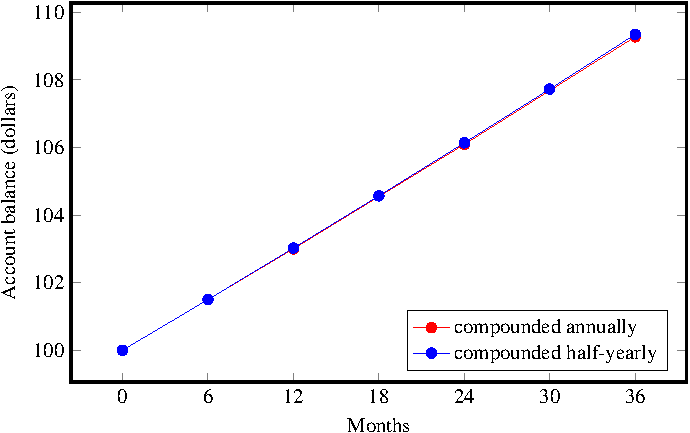
\includegraphics[scale=1.1]{image/11/interest-yearly.pdf}
\caption{%%
  The balance of a savings account within the first three years since
  being opened.  The initial balance is $\$100$ with an interest rate
  of $3\%$ per annum.  The red graph shows the balance when interest
  is compounded once per year.  The blue graph shows the balance when
  interest is compounded twice per year.
}
\label{fig:savings_1year_6months}
\end{figure}

\solutionpart{subex:savings_1year_interest}
Using \Equation{eqn:savings_1year_compounding}, the account balance at
the end of the first year is
\[
B(1)
=
100 \times 1.03^1
=
103
\]
dollars.  The interest that your account would have earned is
$103 - 100 = 3$ dollars.

\solutionpart{subex:savings_1year_doubling_time}
Using the rule of $72$, the doubling time of your account balance is
roughly $72 / 3 = 24$ compounding periods.  As each compounding period
is equivalent to one year, then $24$ compounding periods translate to
$24$ years.  Substitute $t = 24$ into
\Equation{eqn:savings_1year_compounding} to get
\[
B(24)
=
100 \times 1.03^{24}
\approx
203.28
\]
dollars, rounded to the nearest cent.  Substituting $t = 23$ into
\Equation{eqn:savings_1year_compounding} shows that
\[
B(23)
=
100 \times 1.03^{23}
\approx
197.36
\]
dollars, also rounded to the nearest cent.  Therefore the doubling
time of your account balance is at most $24$ years.
\end{solution}
}{}

\begin{example}
\label{eg:savings_quarterly_compounding}
\textbf{Quarterly compounding.}
Suppose that in \Example{eg:savings_6months} interest is compounded
once every three months.
%%
\begin{packedenum}
\item\label{subeg:savings_quarterly_formula}
  Derive a formula for the balance of your account after $t$
  compounding periods.  Produce a graph of your account balance up to
  and including the first three years since you opened the account.
  On the same set of axes, draw the graphs from
  \Subexample{eg:savings_6months}{subeg:savings_6months_balance_formula}
  and
  \Subexercise{ex:savings_once_annually}{subex:savings_1year_formula}
  as comparison.

\item\label{subeg:savings_quarterly_doubling_time}
  Estimate the doubling time of the balance of your savings account.
\end{packedenum}
\end{example}

\begin{solution}
\solutionpart{subeg:savings_quarterly_formula}
The initial balance is $a = 100$ dollars and the interest rate is
$3\%$ per annum.  Since interest is calculated once every three
months, then within a year there would be $12 / 3 = 4$ compounding
periods.  The quarterly interest rate is $3\% / 4 = 0.75\%$, the
quarterly growth rate is $r = 0.75 / 100 = 0.0075$, and the quarterly
growth factor is $b = 1 + 0.0075 = 1.0075$.  If $B(t)$ represents the
account balance after $t$ compounding periods, use
\Theorem{thm:exponential_growth} to write
%%
\begin{equation}
\label{eqn:savings_quarterly_compounding}
B(t)
=
100 \times 1.0075^t.
\end{equation}
%%
The latter equation is graphed in \Figure{fig:savings_quarterly} for
up to the first three years since opening the account.  As a
comparison, the figure also shows the graphs of
\Equation{eqn:compound_interest_a100_b1.015} and of the equation from
\Subexercise{ex:savings_once_annually}{subex:savings_1year_formula}.

\begin{figure}[!htbp]
\centering
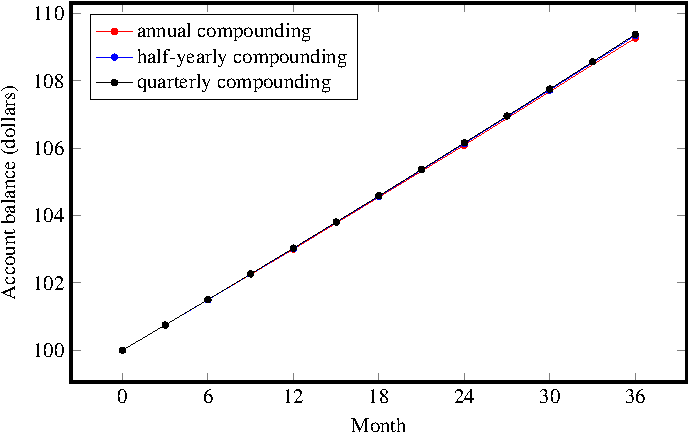
\includegraphics[scale=1.1]{image/11/interest-quarterly.pdf}
\caption{%%
  The balance of a savings account up to the first three years since
  being opened.  The interest rate is $3\%$ per annum.  The red, blue,
  and black graphs show the account balance when interest is
  compounded annually, half-yearly, or every three months,
  respectively.
}
\label{fig:savings_quarterly}
\end{figure}

\solutionpart{subeg:savings_quarterly_doubling_time}
You want to know the amount of time required for the initial balance
of your account to double to $\$200$.  You can use the rule of $72$ to
calculate a rough estimate of the doubling time of your account
balance.  Since the quarterly interest rate is $0.75\%$, the rule of
$72$ tells you that the doubling time of your account balance is
approximately $72 / 0.75 = 96$ compounding periods.  Since each
compounding period corresponds to three months, $96$ compounding
periods translate to $96 \times 3 = 288$ months, which in turn is
equivalent to $288 / 12 = 24$ years.  However, if you substitute
$t = 93$ compounding periods into
\Equation{eqn:savings_quarterly_compounding} you would get
\[
B(93)
=
100 \times 1.0075^{93}
\approx
200.35
\]
dollars, rounded to the nearest cent.  Substituting $t = 92$ into
\Equation{eqn:savings_quarterly_compounding} yields
\[
B(92)
=
100 \times 1.0075^{92}
\approx
198.86
\]
dollars, also rounded to the nearest cent.  Therefore the doubling
time of your account balance is at most $t = 93$ compounding periods,
which is equivalent to $93 \times 3 = 279$ months or
$\frac{93 \times 3}{12} = 23.25$ years.
\end{solution}

\begin{exercise}
\textbf{How much interest?}
In \Example{eg:savings_quarterly_compounding}, how much interest~(in
dollars) would your account earn at the end of the first year?
\end{exercise}

\ifbool{showSolution}{
\begin{solution}
Since each compounding period corresponds to three months, within a
year you have $12 / 3 = 4$ compounding periods.  Substitute $t = 4$
into \Equation{eqn:savings_quarterly_compounding} to see that your
account balance at the end of the first year is approximately
\[
B(4)
=
100 \times 1.0075^4
\approx
103.03
\]
dollars, rounded to the nearest cent.  The amount of interest that
your account would have earned is $103.03 - 100 = 3.03$ dollars.
\end{solution}
}{}

\begin{exercise}
\textbf{Monthly compounding.}
Suppose that in \Example{eg:savings_6months} interest is calculated
once per month.
%%
\begin{packedenum}
\item\label{subex:savings_monthly_formula}
  Derive a formula for the balance of your account after $t$ months.
  Produce a graph of the balance of your account.  On the same set of
  axes, draw the graphs from
  \Subexample{eg:savings_6months}{subeg:savings_6months_balance_formula},
  \Subexercise{ex:savings_once_annually}{subex:savings_1year_formula},
  and
  \Subexample{eg:savings_quarterly_compounding}{subeg:savings_quarterly_formula}.
  The time frame on the horizontal axis should be from the $30$-th
  month up to and including the $36$-th month since opening the
  account.

\item\label{subex:savings_monthly_interest}
  Calculate the amount of interest~(in dollars) that your account
  would earn at the end of the first year.

\item\label{subex:savings_monthly_doubling_time}
  Estimate the doubling time of your account balance.
\end{packedenum}
\end{exercise}

\ifbool{showSolution}{
\begin{solution}
\solutionpart{subex:savings_monthly_formula}
The initial balance is $a = 100$ dollars and the interest rate is
$3\%$ per annum.  Since interest is calculated once a month, the
monthly interest rate is $3\% / 12 = 0.25\%$, the monthly growth rate
is $r = 0.25 / 100 = 0.0025$, and the monthly growth factor is
$b = 1 + 0.0025 = 1.0025$.  Each compounding period corresponds to one
month.  If $B(t)$ represents the balance of your account at the end of
$t$ months, use \Theorem{thm:exponential_growth} to write $B(t)$ as
%%
\begin{equation}
\label{eqn:savings_monthly_balance}
B(t)
=
100 \times 1.0025^t.
\end{equation}
%%
\Figure{fig:savings_monthly_comparison} shows a comparison of the
account balance from the $30$-th month up to the $36$-th month since
opening the account.

\begin{figure}[!htbp]
\centering
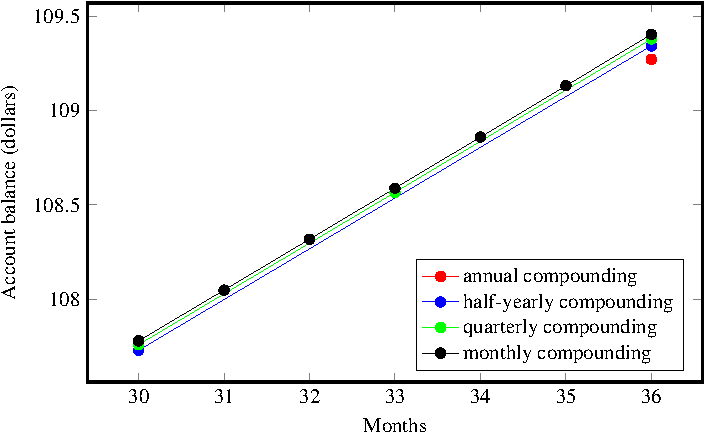
\includegraphics[scale=1.1]{image/11/interest-monthly.pdf}
\caption{%%
  The balance of a savings account from the $30$-th month up to and
  including the $36$-th month since the account was opened.  The
  account has an initial balance of $\$100$ and an interest rate of
  $3\%$ per annum.
}
\label{fig:savings_monthly_comparison}
\end{figure}

\solutionpart{subex:savings_monthly_interest}
Each compounding period corresponds to one month, so within a year you
have $12$ compounding periods.  Substitute $t = 12$ into
\Equation{eqn:savings_monthly_balance} to see that at the end of the
first year your account balance would be approximately
\[
B(12)
=
100 \times 1.0025^{12}
\approx
103.04
\]
dollars, rounded to the nearest cent.  The amount of interest that
your account would have earned is $103.04 - 100 = 3.04$ dollars.

\solutionpart{subex:savings_monthly_doubling_time}
You want to know the amount of time required for the initial account
balance to double to $\$200$.  You can use the rule of $72$ to obtain
a rough estimate of the doubling time.  Since the monthly interest
rate is $0.25\%$, the rule of $72$ tells you that the doubling time is
approximately $72 / 0.25 = 288$ months.  However, substituting
$t = 278$ into \Equation{eqn:savings_monthly_balance} shows that
\[
B(278)
=
100 \times 1.0025^{278}
\approx
200.20
\]
dollars, rounded to the nearest cent.  Furthermore, substituting
$t = 277$ into \Equation{eqn:savings_monthly_balance} yields
\[
B(277)
=
100 \times 1.0025^{277}
\approx
199.70
\]
dollars, also rounded to the nearest cent.  Therefore the doubling
time of your account balance is at most $278$ months, which is
equivalent to approximately $278 / 12 \approx 23.1667$ years, rounded
to four decimal places.
\end{solution}
}{}


\newpage
%%%%%%%%%%%%%%%%%%%%%%%%%%%%%%%%%%%%%%%%%%%%%%%%%%%%%%%%%%%%%%%%%%%%%%%%%%%

\section*{Problem}

\begin{problem}
\item Read the following paper by Raymond Garver:
  \emph{Compound interest}.\footnote{
    Available at the following website:
    \url{http://www.jstor.org/stable/3027766}.
  }

\begin{figure}[!htbp]
\centering
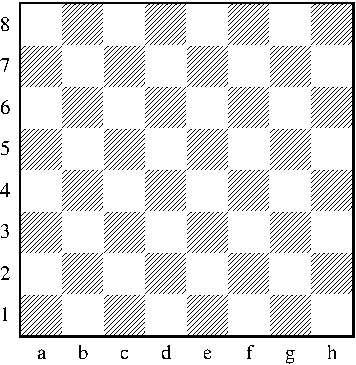
\includegraphics[scale=1.1]{image/11/chessboard.pdf}
\caption{%%
  A standard $8 \times 8$ chessboard.
}
\label{fig:chessboard}
\end{figure}

\item Consider the $64$ squares in the chessboard of
  \Figure{fig:chessboard}, going from left to right, top to bottom.
  You place one grain of sand on the first square.  The number of
  grains of sand you place on the second square is doubled the number
  of grains of sand on the first square.  On the third square, the
  number of grains of sand you deposit is doubled the number of grains
  of sand on the second square.  You continue this doubling process up
  to and including the $64$-th square.
  %%
  \begin{packedenum}
  \item\label{subprob:sand_formula}
    Derive a formula for the number of grains of sand on any given
    square.  Use the formula to calculate the number of grains of sand
    on the $64$-th square.

  \item\label{subprob:sand_neurons_human_brain}
    It is estimated that a human brain contains approximately
    $86 \times 10^9 = 86,000,000,000$ neurons or $86$ billion
    neurons.\footnote{
      See the following paper for further details:
      \url{https://doi.org/10.3389/neuro.09.031.2009}
    }
    How many times must you perform the doubling process above in
    order for the number of grains of sand on a square to be greater
    than $86$ billion?
  \end{packedenum}
\ifbool{showSolution}{
\begin{solution}
\solutionpart{subprob:sand_formula}
Let $t \geq 0$ be the number of times that you perform the doubling
process.  You start off with one grain of sand on the first square so
the number of times you have performed the doubling process is zero.
You perform the doubling process once to obtain the number of grains
of sand for the second square.  To obtain the number of grains of sand
for the third square, you must perform the doubling process three
times.  In general, to obtain the number of grains of sand for the
$n$-th square you must perform the doubling process a total of
$t = n + 1$ times.

Let $G(t)$ represent the number of grains of sand on square number
$t + 1$.  For example, you have $G(0) = 1 = 2^0$ grain of sand on
square number $0 + 1 = 1$.  You have $G(1) = 2 = 2^1$ grains of sand
on square number $1 + 1 = 2$.  On square number $2 + 1 = 3$, you have
$G(2) = 4 = 2^2$ grains of sand.  You have $G(3) = 8 = 2^3 = 8$ grains
of sand on square number $3 + 1 = 4$.  Furthermore, you have
$G(4) = 16 = 2^4$ grains of sand on square number $4 + 1 = 5$.  In
general, you have $G(t) = 2^t$ grains of sand on square number
$t + 1$.

You can also derive the equation $G(t) = 2^t$ as follows.  The initial
amount of sand is $a = 1$ grain.  The constant percentage rate of
growth is $100\%$ so the rate of growth is $r = 1$, hence the growth
factor is $b = 1 + 1 = 2$.  Using \Theorem{thm:exponential_growth},
you can write
\[
G(t)
=
ab^t
=
1 \times 2^t
=
2^t.
\]
You have $G(63)$ grains of sand on square number $63 + 1 = 64$.
Therefore the $64$-th square would have
\[
G(63)
=
2^{63}
=
9,223,372,036,854,775,808
\]
grains of sand.

\solutionpart{subprob:sand_neurons_human_brain}
For $t = 36$ you have
\[
G(36)
=
2^{36}
=
68,719,476,736
\]
grains of sand on square $36 + 1 = 37$.  For $t = 37$, you have
\[
G(37)
=
2^{37}
=
137,438,953,472
\]
grains of sand or over $137$ billion grains of sand on square
$37 + 1 = 38$.  Therefore you must perform the doubling process at
least $37$ times in order for a square to contain over $86$ billion
grains of sand.
\end{solution}
}{}

\item Recall that the number $e = 2.718281\dots$ is an irrational
  number.  This problem will help you to understand how the number $e$
  is related to compound interest.  Suppose that at the start of a
  year you opened a savings account and deposit $\$1$ into the
  account.  You leave the account open for a full year without
  depositing any more money into it nor withdrawing any money out of
  the account.  Suppose that the account has an interest rate of
  $100\%$ per annum.
  %%
  \begin{packedenum}
  \item\label{subprob:e_balance_formula}
    Let $n$ be the number of times that interest is calculated during
    a year.  If $B(n)$ represents the balance of your account at the
    end of the first year, show that $B(n)$ can be written as
    %%
    \begin{equation}
    \label{eqn:e_savings_first_year_n_compounding}
    B(n)
    =
    \parenthesis*{
      1 + \frac{1}{n}
    }^n.
    \end{equation}

  \item\label{subprob:e_balance_up_to_12_compounding}
    You can use \Equation{eqn:e_savings_first_year_n_compounding} to
    investigate the effect of the number $n$ of interest compounding
    per annum on the balance $B(n)$ of your account at the end of the
    first year.  Consider the case of $n = 1$ interest calculation per
    annum.  What would be your account balance at the end of the first
    year?  If interest is calculated $n = 2$ times per annum, what
    would the value of $B(n)$ be?  Repeat the same calculation for
    $n = 3$, $n = 4$, and so on, up to $n = 12$.  Organise your
    results as a table with three columns and as many rows as
    neccessary.  Going from left to right, the first column should
    contain the numbers $n$ of times that interest is calculated per
    annum.  Next, the second column should contain the corresponding
    growth factors.  Finally, the third column should contain the
    corresponding values of $B(n)$.  Produce two graphs of the data in
    your table.  One graph should show the value of $n$ versus the
    growth factor.  The second graph should show the value of $n$
    versus $B(n)$.

  \item\label{subprob:e_balance_up_to_1200_compounding}
    Start at $n = 12$ compoundings per annum and increase $n$ by $12$
    each time up to $100$ times.  Thus you would have the sequence
    %%
    \begin{equation}
    \label{eqn:e_balance_up_to_1200_compounding}
    \seq{\pair{12}{24}}{\pair{36}{48}}{1200}
    \end{equation}
    %%
    of compoundings per annum.  For each of the numbers
    in~\eqref{eqn:e_balance_up_to_1200_compounding}, calculate the
    corresponding growth factor.  Use your results to produce a graph
    of the number of compoundings per annum versus the growth factor.
    Furthermore, for each of the numbers
    in~\eqref{eqn:e_balance_up_to_1200_compounding}, calculate the
    corresponding account balance at the end of the first year.  Also
    use your results to produce a graph of the number of compoundings
    per annum versus the account balance at the end of the first
    year.

  \item\label{subprob:e_balance_limit_of_growth_factor_balance}
    Based on \Equation{eqn:e_savings_first_year_n_compounding} and
    your graphs from \Part{subprob:e_balance_up_to_1200_compounding},
    describe the value of the growth factor as the number $n$ of
    compoundings per annum gets larger and larger.  Furthermore,
    describe the value of $B(n)$ as $n$ gets larger and larger.
    Provide an interpretation of your results.

  \item\label{subprob:e_balance_continuous_compounding}
    As the number of compounding periods per annum continually grows
    larger and larger, you have a situation called
    \emph{continuous compounding}.  The formula for continuous
    compounding is written as
    \[
    B(t)
    =
    P e^{rt}
    \]
    where $P$ is the initial balance or \emph{principal}, $r$ is the
    interest rate per annum written as a decimal, and $t$ is the
    number of years.  (The formula sounds like ``pert''.)  Calculate
    your account balance at the end of the first year if interest is
    continuously compounded.
  \end{packedenum}
\ifbool{showSolution}{
\begin{solution}
\solutionpart{subprob:e_balance_formula}
The initial balance is $a = 1$ dollar.  Since there are $n$
compounding periods per year, at each compounding period the rate you
use for interest calculation is $100 / n$ percent.  Divide this number
by $100$ to get the constant growth rate of
\[
r
=
\frac{100}{n} \times \frac{1}{100}
=
\frac{1}{n}.
\]
Then the growth factor is $b = 1 + r = 1 + \frac{1}{n}$.  If $B(t)$
represents the account balance at the end of the $t$-th compounding
period, use \Theorem{thm:exponential_growth} to write
%%
\begin{align*}
B(t)
&=
1 \times \parenthesis*{1 + \frac{1}{n}}^t \\[4pt]
&=
\parenthesis*{1 + \frac{1}{n}}^t.
\end{align*}
%%
You have $n$ compounding periods per year, so the account balance at
the end of the first year is $B(n)$, which can be written as
\[
B(n)
=
\parenthesis*{1 + \frac{1}{n}}^n
\]
as required.

\solutionpart{subprob:e_balance_up_to_12_compounding}
See \Table{tab:e_balance_up_to_12_compounding} and
\Figure{fig:e_balance_up_to_12_compounding}.

\begin{table}[!htbp]
\centering
\begin{tabular}{rcc}                    \toprule
$n$  & $1 + \frac{1}{n}$ & $B(n)$     \\\midrule
$1$  & $2.000000$        & $2.000000$ \\
$2$  & $1.500000$        & $2.250000$ \\
$3$  & $1.333333$        & $2.370370$ \\
$4$  & $1.250000$        & $2.441406$ \\
$5$  & $1.200000$        & $2.488320$ \\
$6$  & $1.166667$        & $2.521626$ \\
$7$  & $1.142857$        & $2.546500$ \\
$8$  & $1.125000$        & $2.565785$ \\
$9$  & $1.111111$        & $2.581175$ \\
$10$ & $1.100000$        & $2.593742$ \\
$11$ & $1.090909$        & $2.604199$ \\
$12$ & $1.083333$        & $2.613035$ \\\bottomrule
\end{tabular}

\caption{%%
  The effect of the number $n$ of compounding periods per annum on the
  account balance $B(n)$ at the end of the first year.  Here $B(n)$ is
  defined as in \Equation{eqn:e_savings_first_year_n_compounding}.  The
  number $1 + \frac{1}{n}$ is the growth factor.  All numbers in the
  middle and right-most columns have been rounded to six decimal
  places.
}
\label{tab:e_balance_up_to_12_compounding}
\end{table}

\begin{figure}[!htbp]
\centering
\subfigure[]{
  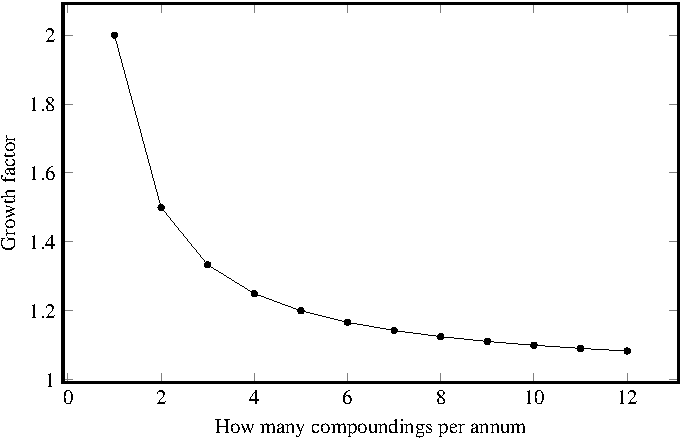
\includegraphics[scale=1.1]{image/11/e-12-growth-factor.pdf}
}
%%
%%
\subfigure[]{
  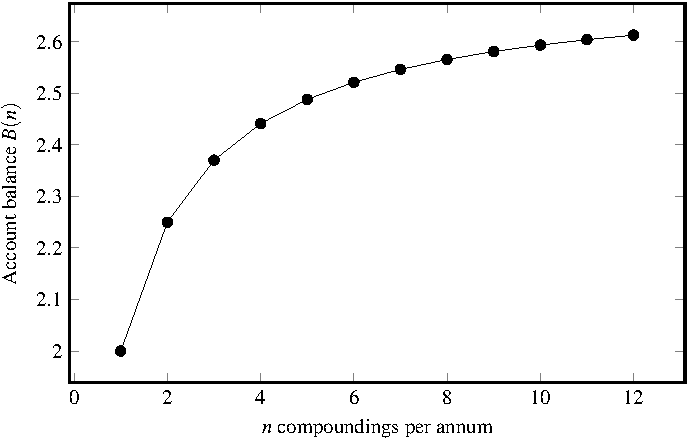
\includegraphics[scale=1.1]{image/11/e-12-balance.pdf}
}
\caption{%%
  The effect of the number of compounding periods per annum on
  (a)~the growth factor and (b)~the account balance at the end of the
  first year.  Data are from
  \Table{tab:e_balance_up_to_12_compounding}.
}
\label{fig:e_balance_up_to_12_compounding}
\end{figure}

\solutionpart{subprob:e_balance_up_to_1200_compounding}
See \Figure{fig:e_savings_up_to_1200_compounding}.

\begin{figure}[!htbp]
\centering
\subfigure[]{
  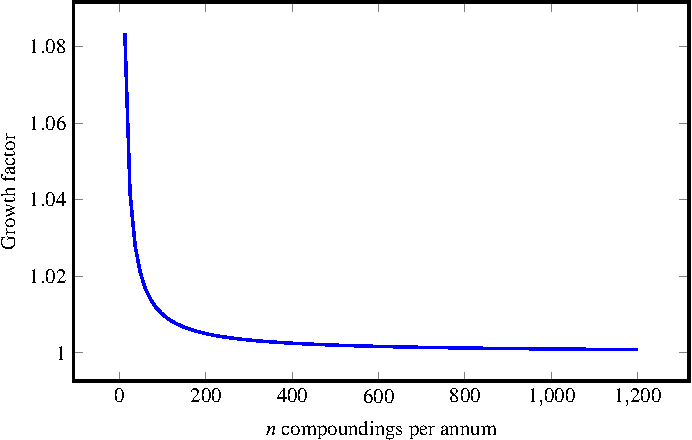
\includegraphics[scale=1.1]{image/11/e-1200-growth-factor.pdf}
  \label{subfig:e_savings_1200_growth_factor}
}
%%
%%
\subfigure[]{
  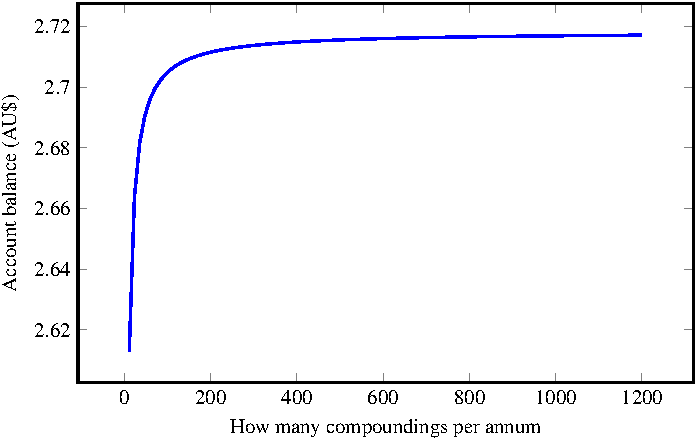
\includegraphics[scale=1.1]{image/11/e-1200-balance.pdf}
  \label{subfig:e_savings_1200_balance}
}
\caption{%%
  The effect of the number $n$ of compoundings per annum on (a)~the
  growth factor and (b)~the account balance at the end of the first
  year.  The number $n$ is up to $1200$ compoundings per annum.
}
\label{fig:e_savings_up_to_1200_compounding}
\end{figure}

\begin{figure}[!htbp]
\centering
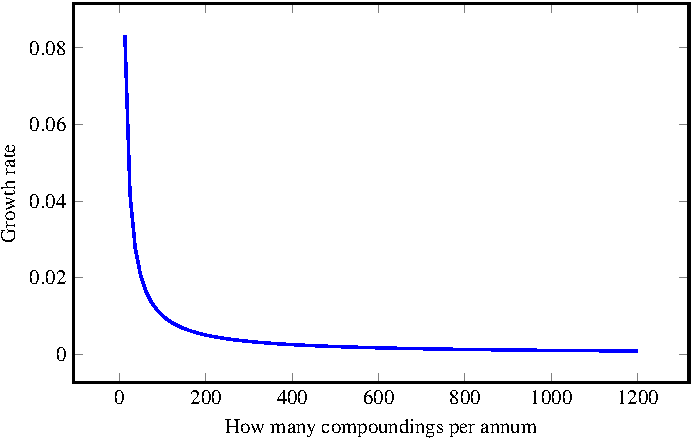
\includegraphics[scale=1.1]{image/11/e-1200-growth-rate.pdf}
\caption{%%
  The effect of the number $n$ of interest compoundings per annum on
  the growth rate $f(n) = 1 / n$.  Since the interest rate is $100\%$
  per annum, the interest rate as a decimal is $100 / 100 = 1$, which
  is the numerator of $f(n)$.  In other words, the function $f(n)$
  tells you the growth rate when interest is calculated $n$ times each
  year.
}
\label{fig:e_saving_1200_growth_rate}
\end{figure}

\solutionpart{subprob:e_balance_limit_of_growth_factor_balance}
Consider the growth factor $g(n) = 1 + \frac{1}{n}$, where $n$
represents the number of interest compoundings per annum.  As $n$
becomes larger and larger, the growth rate $1 / n$ becomes smaller and
smaller and approaches zero.  This effect can be seen in
\Figure{fig:e_saving_1200_growth_rate}.  That is, as $n$ gets larger
and larger the growth factor $g(n)$ gets closer and closer to the
value of $1$; see \Figure{subfig:e_savings_1200_growth_factor}.
Therefore the account balance $B(n)$ at the end of the first year gets
closer and closer to a fixed number.  From
\Figure{subfig:e_savings_1200_balance}, the fixed number is
approximately $2.72$.  What do these results mean?  Suppose you have a
fixed annual interest rate and a fixed initial account balance.  No
matter how many times that interest is calculated per year, your
account balance at the end of the first year will never grow as large
and you want.

\solutionpart{subprob:e_balance_continuous_compounding}
The initial balance is $P = 1$ dollar, the annual interest rate is
$100\%$ so that $r = 100 / 100 = 1$, and $t = 1$ year.  Using the
formula for continuous compounding, your account balance at the end of
the first year is
\[
B(1)
=
1 \times e^{1 \times 1}
=
e
\]
dollars.
\end{solution}
}{}

\item In episode~6, season~1 of \emph{Futurama}~(1999), Fry learnt
  that due to compound interest his account balance had grown to
  billions of dollars.  You can watch the relevant clip at:
  \url{https://youtu.be/f2Wi6AoArV0}.  Determine the initial balance
  of Fry's account, the annual growth rate of the account balance, and
  the number of years for which the balance had been left to grow.
  Determine the formula that the bank teller used to approximate Fry's
  current account balance and use the formula to calculate Fry's
  current account balance, rounded to the nearest cent.  If the
  interest on Fry's account had been continuously compounded, what
  would Fry's account balance be at the end of the given number of
  compounding years?
\ifbool{showSolution}{
\begin{solution}
Fry had an initial account balance of $\cent{93}$ or $\$0.93$.  The
interest is $2.25\%$ per annum, so the annual growth rate is
$r = 2.25 / 100 = 0.0225$.  The account balance had been left to
grow for $1000$ years.  The bank teller used the following formula to
approximate Fry's account balance:
\[
B(t)
=
0.93 \times 1.0225^t
\]
assuming that interest is calculated once per annum.  Using the above
formula, Fry's account balance after $t = 1000$ years is
\[
B(1000)
=
0.93 \times 1.0225^{1000}
\approx
4,283,508,449.71
\]
dollars, rounded to the nearest cent.  This can also be rounded to
$4.3$ billion dollars.  If interest had been continuously compounded,
Fry's account balance at the end of $1000$ years would be
\[
0.93 e^{0.0225 \times 1000}
\approx
5,496,785,518.61
\]
dollars, rounded to the nearest cent.
\end{solution}
}{}

\begin{table}[!htbp]
\centering
\begin{tabular}{ccc}                    \toprule
Day & Frond no. & Daily growth factor \\\midrule
$1$ & $103$     & ---                 \\
$2$ & $126$ \\
$3$ & $144$ \\
$4$ & $161$ \\
$5$ & $190$ \\
$6$ & $218$ \\
$7$ & $248$ \\
$8$ & $279$ \\
$9$ & $334$ \\\bottomrule
\end{tabular}

\caption{%%
  The experimental number of fronds in a colony of duckweeds, counted
  each day for nine consecutive days.  Before the first day, the
  colony had been exposed to $12$ hours of light per day for three
  consecutive days.  The missing entries should contain the daily
  growth factors.
}
\label{tab:duckweed_frond12_missing}
\end{table}

\item\label{prob:duckweeds}
  The mathematical formulae that govern compound interest are also
  found in the early stages of the growth of plants.  In~1929, Eric
  Ashby showed via a number of experiments that the growth of
  duckweeds followed the formula for continuous compounding.\footnote{
    See the following paper for further details:
    \url{http://www.jstor.org/stable/43237140}.
  }
  In one experiment, Ashby exposed a colony of duckweeds to $12$ hours
  of light per day for three consecutive days.  After the three days,
  the duckweeds were allowed to grow for nine consecutive days.
  During each of the nine days, the number of fronds~(the leaves of
  the duckweeds) were counted and the results are given in
  \Table{tab:duckweed_frond12_missing}.
  %%
  \begin{packedenum}
  \item\label{subprob:duckweeds_growth_factor}
    Graph the data in \Table{tab:duckweed_frond12_missing} as a
    scatter plot.  From \Table{tab:duckweed_frond12_missing}, suppose
    that the initial number of fronds is $a = 103$.  Starting from the
    second day onwards, define the \emph{daily growth factor} as the
    number of fronds of the current day divided by the number of
    fronds of the previous day.  Use this procedure to fill in the
    missing entries in \Table{tab:duckweed_frond12_missing}.  The
    daily growth factor for day~$1$ should be blank.  If the data in
    \Table{tab:duckweed_frond12_missing} perfectly follow the model of
    exponential growth, what do you expect all the daily growth
    factors to be like?  What can you conclude from the daily growth
    factors of \Table{tab:duckweed_frond12_missing}?

  \item\label{subprob:duckweeds_growth_factor_estimate}
    Using the daily growth factors
    from \Part{subprob:duckweeds_growth_factor}, you can obtain a
    rough estimate of the growth factor of the frond numbers by
    calculating the mean of the daily growth factors.  Use your
    estimated growth factor to derive a formula for the growth of the
    number of fronds.  Produce a graph of the day number versus the
    experimental number of fronds.  On the same set of axes, draw a
    graph of your growth formula.

  \item\label{subprob:duckweeds_growth_factor_exponential}
    Ashby calculated that given an initial population of $a = 100$
    fronds and a growth rate of $r = 0.127$, the number $f(t)$ of
    fronds on day $t$ can be written as
    %%
    \begin{equation}
    \label{eqn:frond_numbers_Ashby_formula}
    f(t)
    =
    100 e^{0.127t}.
    \end{equation}
    %%
    Note the irrational number $e$.  Produce a table with four columns
    and as many rows as necessary.  The first row should contain the
    column headings.  Going from left to right, the first two columns
    should contain the same data as in the first two columns of
    \Table{tab:duckweed_frond12_missing}.  The third column should
    contain the frond numbers as calculated using your formula
    from \Part{subprob:duckweeds_growth_factor_estimate}.  Finally,
    the fourth column should contain the frond numbers as calculated
    using Ashby's \Equation{eqn:frond_numbers_Ashby_formula}.  Add to
    the graph in \Part{subprob:duckweeds_growth_factor_estimate} a
    graph of \Equation{eqn:frond_numbers_Ashby_formula}.  By using the
    root mean square error~(i.e.~the RMS error), explain which of
    \Equation{eqn:frond_numbers_Ashby_formula} and your equation
    from \Part{subprob:duckweeds_growth_factor_estimate} is better at
    modelling the frond numbers listed in
    \Table{tab:duckweed_frond12_missing}.
  \end{packedenum}
\ifbool{showSolution}{
\begin{solution}
\solutionpart{subprob:duckweeds_growth_factor}
See \Figure{fig:frond12_theory_data} and
\Table{tab:duckweed_frond12_complete}.  If the data in
\Table{tab:duckweed_frond12_missing} were to perfectly follow the
model of exponential growth, then the daily growth factors for the
data should all be the same.  In fact, the daily growth factors would
be the same as the growth factor of an exponential growth model.
However, as shown in \Table{tab:duckweed_frond12_complete} the daily
growth factors for the data are not all the same.  The daily growth
factors are similar in terms of the first decimal digits, but they are
not approximately the same in the second decimal digits.  You can
conclude from the daily growth factors that the data in
\Table{tab:duckweed_frond12_missing} do not perfectly follow an
exponential growth model.  However, the daily growth factors are
nearly the same in the first decimal digits, and the scatter plot of
the data seems to show an exponential-like growth, that you can
attempt to model the data with a formula for exponential growth.

\begin{table}[!htbp]
\centering
\begin{tabular}{ccc}                    \toprule
Day & Frond no. & Daily growth factor \\\midrule
$1$ & $103$     & ---        \\
$2$ & $126$     & $1.223301$ \\
$3$ & $144$     & $1.142857$ \\
$4$ & $161$     & $1.118056$ \\
$5$ & $190$     & $1.180124$ \\
$6$ & $218$     & $1.147368$ \\
$7$ & $248$     & $1.137615$ \\
$8$ & $279$     & $1.125000$ \\
$9$ & $334$     & $1.197133$ \\\bottomrule
\end{tabular}

\caption{%%
  The experimental number of fronds in a colony of duckweeds, counted
  each day for nine consecutive days.  Before the first day, the
  colony had been exposed to $12$ hours of light per day for three
  consecutive days.  This is the same as
  \Table{tab:duckweed_frond12_missing} except that missing entries
  have been filled in.  All numbers in the column for daily growth
  factor have been rounded to six decimal places.
}
\label{tab:duckweed_frond12_complete}
\end{table}

\solutionpart{subprob:duckweeds_growth_factor_estimate}
You can estimate the growth factor for the number of fronds by
calculating the mean of the daily growth factors.  Doing so, the
growth factor is estimated to be $b = 1.158932$, rounded to six
decimal places.  The initial number of fronds is $a = 103$.  If $F(t)$
denotes the number of fronds on day $t$, then you can write $F(t)$ as
%%
\begin{equation}
\label{eqn:fronds_formula_average_growth_factor}
F(t)
=
103 \times 1.158932^{t - 1}.
\end{equation}
%%
Note the exponent of $t - 1$.  You have this exponent because if you
substitute $t = 1$ into
\Equation{eqn:fronds_formula_average_growth_factor}, then you should
obtain the initial number of fronds:
%%
\begin{align*}
F(1)
&=
103 \times 1.158932^{1 - 1} \\[4pt]
&=
103 \times 1.158932^0 \\[4pt]
&=
103.
\end{align*}
%%
\Figure{fig:frond12_theory_data} shows a graph of
\Equation{eqn:fronds_formula_average_growth_factor} together with the
experimental data from \Table{tab:duckweed_frond12_missing}.

\begin{figure}[!htbp]
\centering
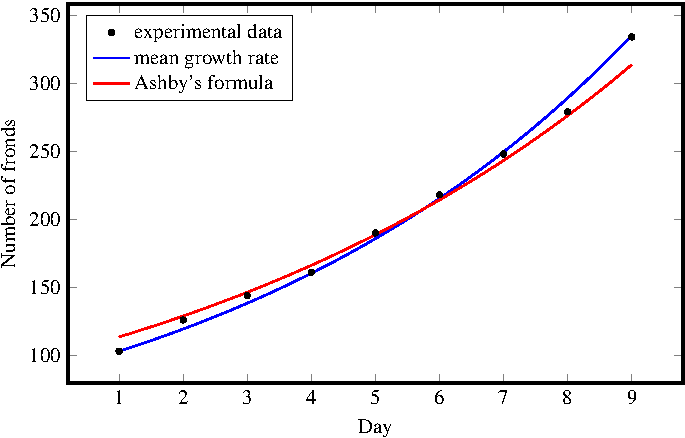
\includegraphics[scale=1.1]{image/11/frond12-estimated-b.pdf}
\caption{%%
  A comparison of the observed frond numbers versus the predicted
  frond numbers as given by
  \Equations{eqn:frond_numbers_Ashby_formula}{eqn:fronds_formula_average_growth_factor}.
  The black dots
  represent the experimental data from
  \Table{tab:duckweed_frond12_missing}.  The blue curve is a graph of
  \Equation{eqn:fronds_formula_average_growth_factor}, which is based
  on the mean growth rate.  The red curve is a graph of Ashby's
  \Equation{eqn:frond_numbers_Ashby_formula}.
}
\label{fig:frond12_theory_data}
\end{figure}

\solutionpart{subprob:duckweeds_growth_factor_exponential}
\Table{tab:frond12_compare_mean_Ashby} and
\Figure{fig:frond12_theory_data} compare the observed frond numbers
with the predicted frond numbers.  The table also shows the squared
errors of the predictions.  Using these squared errors, the RMS error
of \Equation{eqn:fronds_formula_average_growth_factor} is
$4.8256$, which is smaller than the RMS error of $8.2572$ of Ashby's
\Equation{eqn:frond_numbers_Ashby_formula}, both numbers rounded to
four decimal places.  Based on the RMS errors, you may conclude that
\Equation{eqn:fronds_formula_average_growth_factor} is better than
Ashby's formula at modelling the observed frond numbers.

\begin{table}[!htbp]
\centering
\begin{tabular}{cccc}                            \toprule
    &          & \multicolumn{2}{c}{Prediction} \\
  \cmidrule{3-4}
Day & Observed & $F(t)$    & Ashby   \\\midrule
$1$ & $103$    & $103.0$   & $113.5$ \\[4pt]
$2$ & $126$    & $119.4$   & $128.9$ \\[4pt]
$3$ & $144$    & $138.3$   & $146.4$ \\[4pt]
$4$ & $161$    & $160.3$   & $166.2$ \\[4pt]
$5$ & $190$    & $185.8$   & $188.7$ \\[4pt]
$6$ & $218$    & $215.3$   & $214.3$ \\[4pt]
$7$ & $248$    & $249.6$   & $243.3$ \\[4pt]
$8$ & $279$    & $289.2$   & $276.2$ \\[4pt]
$9$ & $334$    & $335.2$   & $313.6$ \\\bottomrule
\end{tabular}

\caption{%%
  Comparison of the observed frond numbers versus the predicted frond
  numbers.  The predicted frond numbers as calculated by
  \Equations{eqn:fronds_formula_average_growth_factor}{eqn:frond_numbers_Ashby_formula}
  are listed, respectively, in the third and fourth columns.  These
  numbers have been rounded to one decimal place.  The fifth and sixth
  columns show the squared errors of the predictions.  Although the
  squared errors have been rounded to four decimal places in order to
  fit the table, you should not round these intermediate results when
  you calculate the RMS error.
}
\label{tab:frond12_compare_mean_Ashby}
\end{table}

\end{solution}
}{}

\item A \emph{binary number} is a number that is written in terms of
  $1$~(one) and $0$~(zero).  Something such as $10011010$ is a binary
  number and can be used to represent a non-negative integer inside a
  digital computer.  In fact, your computer and smart phone
  essentially process binary numbers.  The number of digits in a
  binary number is called the \emph{number of bits}.  For instance,
  the binary number $10011010$ has eight bits.
  %%
  \begin{packedenum}
  \item\label{subprob:binary_to_decimal}
    Here is a procedure to convert a binary number to a non-negative
    integer.  Suppose you have a binary number written as
    %%
    \begin{equation}
    \label{eqn:binary_general_number}
    b_{n-1} b_{n-2} \cdots b_2 b_1 b_0
    \end{equation}
    %%
    where the number of bits is $n$ and each $b_i$~(from $i = 0$ to
    $i = n - 1$) is either $0$ or $1$.  In the case of the binary
    $10011010$, you have $n = 8$ because there are eight bits and each
    $b_i$ is
    %%
    \begin{equation}
    \label{eqn:binary_10011010}
    b_7 = 1\comma
    b_6 = 0\comma
    b_5 = 0\comma
    b_4 = 1\comma
    b_3 = 1\comma
    b_2 = 0\comma
    b_1 = 1\comma
    b_0 = 0.
    \end{equation}
    %%
    To convert the binary number~\eqref{eqn:binary_general_number} to
    a non-negative integer, you calculate the sum
    %%
    \begin{equation}
    \label{eqn:binary_to_decimal_formula}
    \sum_{i=0}^{n-1} b_i 2^i
    =
    b_{n-1} 2^{n-1} + b_{n-2} 2^{n-2} + \cdots
    + b_2 2^2 + b_1 2^1 + b_0 2^0.
    \end{equation}
    %%
    For instance, the binary number $10011010$ as defined
    in~\eqref{eqn:binary_10011010} can be converted to a non-negative
    integer as
    %%
    \begin{align*}
    &b_7 2^7 + b_6 2^6 + b_5 2^5 + b_4 2^4
      + b_3 2^3 + b_2 2^2 + b_1 2^1 + b_0 2^0 \\[4pt]
    &=
    1 \times 2^7 + 0 \times 2^6 + 0 \times 2^5 + 1 \times 2^4
    + 1 \times 2^3 + 0 \times 2^2 + 1 \times 2^1 + 0 \times 2^0 \\[4pt]
    &=
    2^7 + 2^4 + 2^3 + 2^1 \\[4pt]
    &=
    128 + 16 + 8 + 2 \\[4pt]
    &=
    154.
    \end{align*}
    %%
    Thus the binary number $10011010$ represents the integer $154$.
    Use \Equation{eqn:binary_to_decimal_formula} to convert the binary
    numbers $10100101$, $1001$, and $00000000$ to non-negative
    integers.

  \item\label{subprob:binary_4_bits}
    Given one bit, the possible non-negative integers that can be
    represented with one bit are $0$ and $1$.  All possible binary
    strings with two bits are: $00$, $01$, $10$, and $11$.  At three
    bits, the possible binary strings are: $000$, $001$, $010$, $011$,
    $100$, $101$, $110$, and $111$.  Determine all possible binary
    strings with four bits and the corresponding non-negative integer
    that each binary string represents.

  \item\label{subprob:binary_how_many_integers}
    If a binary number has one bit, how many possible non-negative
    integers can be represented with one bit?  Consider the case of
    two bits.  How many possible non-negative integers can be
    represented with two bits?  How many possible non-negative
    integers can be represented with three bits?  Consider the above
    questions for the case of one, two, three, four, and so on, up to
    ten bits.  Organise your results as a table with two columns and
    as many rows as necessary.  The first row should contain the
    column headings.  The left column should contain the number $n$ of
    bits.  The right column should contain the number of possible
    non-negative integers that can be represented with $n$ bits.
    Analyse your data by using the technique described in
    \Subproblem{prob:duckweeds}{subprob:duckweeds_growth_factor}.

  \item\label{subprob:binary_how_many_integers_formula}
    Use your results from \Part{subprob:binary_how_many_integers} to
    derive a formula for the number of non-negative integers that can
    be represented with $n$ bits.  Verify your formula with the data
    in the table from \Part{subprob:binary_how_many_integers}.
    Determine the largest non-negative integer that can be represented
    with $n$ bits.
  \end{packedenum}
\ifbool{showSolution}{
\begin{solution}
\solutionpart{subprob:binary_to_decimal}
Using \Equation{eqn:binary_to_decimal_formula}, the binary number
$10100101$ can be converted to a non-negative integer as
%%
\begin{align*}
&b_7 2^7 + b_6 2^6 + b_5 2^5 + b_4 2^4
  + b_3 2^3 + b_2 2^2 + b_1 2^1 + b_0 2^0 \\[4pt]
&=
1 \times 2^7 + 0 \times 2^6 + 1 \times 2^5 + 0 \times 2^4
  + 0 \times 2^3 + 1 \times 2^2 + 0 \times 2^1 + 1 \times 2^0 \\[4pt]
&=
2^7 + 2^5 + 2^2 + 2^0 \\[4pt]
&=
128 + 32 + 4 + 1 \\[4pt]
&=
165.
\end{align*}
%%
The binary number $1001$ represents the non-negative integer
%%
\begin{align*}
&b_3 2^3 + b_2 2^2 + b_1 2^1 + b_0 2^0 \\[4pt]
&=
1 \times 2^3 + 0 \times 2^2 + 0 \times 2^1 + 1 \times 2^0 \\[4pt]
&=
2^3 + 2^0 \\[4pt]
&=
8 + 1 \\[4pt]
&=
9.
\end{align*}
%%
The binary number $00000000$ represents the non-negative integer
%%
\begin{align*}
&b_7 2^7 + b_6 2^6 + b_5 2^5 + b_4 2^4
  + b_3 2^3 + b_2 2^2 + b_1 2^1 + b_0 2^0 \\[4pt]
&=
0 \times 2^7 + 0 \times 2^6 + 0 \times 2^5 + 0 \times 2^4
  + 0 \times 2^3 + 0 \times 2^2 + 0 \times 2^1 + 0 \times 2^0 \\[4pt]
&=
0.
\end{align*}

\solutionpart{subprob:binary_4_bits}
See \Table{tab:binary_4_bits}.

\begin{table}[!htbp]
\centering
\begin{tabular}{cc} \toprule
Binary & Integer \\\midrule
$0000$ & $0$     \\
$0001$ & $1$     \\
$0010$ & $2$     \\
$0011$ & $3$     \\
$0100$ & $4$     \\
$0101$ & $5$     \\
$0110$ & $6$     \\
$0111$ & $7$     \\
$1000$ & $8$     \\
$1001$ & $9$     \\
$1010$ & $10$    \\
$1011$ & $11$    \\
$1100$ & $12$    \\
$1101$ & $13$    \\
$1110$ & $14$    \\
$1111$ & $15$    \\\bottomrule
\end{tabular}

\caption{%%
  All possible binary strings with four bits.  Each binary string
  corresponds to a non-negative integer.
}
\label{tab:binary_4_bits}
\end{table}

\solutionpart{subprob:binary_how_many_integers}
See \Table{tab:binary_how_many_integers}.

\begin{table}[!htbp]
\centering
\begin{tabular}{ccrc}                                           \toprule
Bits & How many integers & Growth factor    & Largest integer \\\midrule
$1$  & $2$               & ---              & $1$             \\[4pt]
$2$  & $4$               & $4 / 2 = 2$      & $3$             \\[4pt]
$3$  & $8$               & $8 / 4 = 2$      & $7$             \\[4pt]
$4$  & $16$              & $16 / 8 = 2$     & $15$            \\[4pt]
$5$  & $32$              & $32 / 16 = 2$    & $31$            \\[4pt]
$6$  & $64$              & $64 / 32 = 2$    & $63$            \\[4pt]
$7$  & $128$             & $128 / 64 = 2$   & $127$           \\[4pt]
$8$  & $256$             & $256 / 128 = 2$  & $255$           \\[4pt]
$9$  & $512$             & $512 / 256 = 2$  & $511$           \\[4pt]
$10$ & $1024$            & $1024 / 512 = 2$ & $1023$          \\\bottomrule
\end{tabular}

\caption{%%
  The number of non-negative integers that can be represented with a
  given number of bits.  Going from left to right, the third column
  contains the consecutive growth factors.  Starting from the row with
  two bits downwards, the growth factor for the row is defined as the
  number of non-negative integers that can be represented with $n$
  bits divided by the number of non-negative integers that can be
  represented with $n - 1$ bits.  The right-most column contains the
  largest non-negative integer that can be represented with $n$ bits.
}
\label{tab:binary_how_many_integers}
\end{table}

\solutionpart{subprob:binary_how_many_integers_formula}
\Table{tab:binary_how_many_integers} shows that adding an extra bit
will increase the number of possible non-negative integers by a factor
of $2$.  For instance, starting at $1$ bit you have $2$ possible
non-negative integers.  Adding another bit will result in $2$ bits,
but the number of possible non-negative integers is now
$2 \times 2 = 2^2$.  Going to $3$ bits, the number of possible
non-negative integers is now $2^2 \times 2 = 2^3$.  At $4$ bits, the
number of possible non-negative integers is $2^3 \times 2 = 2^4$.  In
general, the number of possible non-negative integers that can be
represented with $n$ bits is $2^n$.  At $n$ bits, the integer
$0$~(zero) is represented as $000 \cdots 0$, i.e.~a string of $n$
zeros.  In counting the number of possible non-negative integers, you
must take into account the integer zero.  Thus the largest
non-negative integer that can be represented with $n$ bits is
$2^n - 1$.
\end{solution}
}{}

\begin{table}[!htbp]
\centering
\begin{tabular}{cccrrccc} \toprule
Time & Decayed & Remaining &&& Time & Decayed & Remaining \\\midrule
$0$  & $0$     & $1000$    &&& $22$ & $4$     & $20$      \\
$1$  & $165$   & $835$     &&& $23$ & $4$     & $16$      \\
$2$  & $157$   & $678$     &&& $24$ & $2$     & $14$      \\
$3$  & $108$   & $570$     &&& $25$ & $1$     & $13$      \\
$4$  & $112$   & $458$     &&& $26$ & $1$     & $12$      \\
$5$  & $72$    & $386$     &&& $27$ & $2$     & $10$      \\
$6$  & $61$    & $325$     &&& $28$ & $2$     & $8$       \\
$7$  & $57$    & $268$     &&& $29$ & $0$     & $8$       \\
$8$  & $43$    & $225$     &&& $30$ & $2$     & $6$       \\
$9$  & $29$    & $196$     &&& $31$ & $0$     & $6$       \\
$10$ & $33$    & $163$     &&& $32$ & $1$     & $5$       \\
$11$ & $17$    & $146$     &&& $33$ & $1$     & $4$       \\
$12$ & $20$    & $126$     &&& $34$ & $0$     & $4$       \\
$13$ & $17$    & $109$     &&& $35$ & $1$     & $3$       \\
$14$ & $21$    & $88$      &&& $36$ & $0$     & $3$       \\
$15$ & $10$    & $78$      &&& $37$ & $1$     & $2$       \\
$16$ & $15$    & $63$      &&& $38$ & $1$     & $1$       \\
$17$ & $8$     & $55$      &&& $39$ & $0$     & $1$       \\
$18$ & $12$    & $43$      &&& $40$ & $0$     & $1$       \\
$19$ & $3$     & $40$      &&& $41$ & $0$     & $1$       \\
$20$ & $11$    & $29$      &&& $42$ & $1$     & $0$       \\
$21$ & $5$     & $24$ \\\bottomrule
\end{tabular}

\caption{%%
  Experimental data for the decay of $1000$ ``radioactive'' dice,
  simulated via a computer.  Time is measured in minutes.  After the
  elapse of each minute, you have $d$ dice that have ``decayed'' since
  the previous minute and the $r$ remaining dice are yet to
  ``decay''.  Note that $d$ is not the same as the total number of
  dice that have ``decayed'' up to the given time.  A die is
  considered to have ``decayed'' if after a roll the top-most face of
  the die shows six pips.
}
\label{tab:radioactive_dice}
\end{table}

\item You can obtain an understanding of radioactive decay and
  half-life by performing a simple dice experiment.\footnote{
    See for example the video:
    \url{https://youtu.be/HRwey6cwGHo}.  The idea of using the
    ``radioactive'' dice experiment to teach radioactive decay and
    half-life seems to originate with J.~L.~Lewis; see the paper:
    \url{https://doi.org/10.1088/0031-9112/13/1/003}.
  }
  For good experimental data, you should use at least $100$ dice.
  However, you will be using the experimental data from $1000$ dice
  that have been generated from a computer simulation.  The computer
  simulation works as follows.  At time $t = 0$ minutes, you have
  $1000$ dice.  After the elapse of one minute~(i.e.~at time $t = 1$
  minute), the $1000$ dice are rolled and you note the number of pips
  on the top-most face of each die.  If the top-most face of a die
  shows six pips, then you move the die to a pile labelled
  ``decayed''.  The remaining dice that do not have six pips on their
  respective top-most faces are not yet ``decayed''.  After the elapse
  of another minute~(i.e.~at time $t = 2$ minutes), the remaining
  ``non-decayed'' dice from time $t = 1$ are rolled and you note the
  number of pips on the top-most face of each die.  If a die shows six
  pips on its top-most face, you move the die to the ``decayed'' pile
  and the remaining dice are yet to ``decay''.  Repeat the process
  until all dice have ``decayed''.  \Table{tab:radioactive_dice} shows
  the data from one run of the above experiment with $1000$
  ``radioactive'' dice~(the dice were not actually radioactive).
  %%
  \begin{packedenum}
  \item\label{subprob:radioactive_dice_graph_remaining}
    Produce a scatter plot of the number of minutes that have elapsed
    versus the number of remaining ``undecayed'' dice.  How much time
    was required for all the $1000$ dice to be in the ``decay'' state?

  \item\label{subprob:radioactive_dice_cumulative_decayed}
    In \Table{tab:radioactive_dice}, note the two columns with the
    heading ``Decayed''.  Each row shows the number of dice that have
    ``decayed'' since the previous minute.  For example, from time
    $t = 4$ to $t = 5$ you have $72$ dice that have ``decayed'' during
    that one minute interval.  However, what you want is the
    cumulative~(or running) sum of all dice that have decayed up to
    any given time.  Create a column for the cumulative sum of
    ``decayed'' dice.  Plot the cumulative sum of ``decayed'' dice
    versus time together with the graph
    from \Part{subprob:radioactive_dice_graph_remaining}.

  \item\label{subprob:radioactive_dice_decay_constant}
    Let $t_{1/2}$ be the half-life of an exponential decay model.  If
    $\lambda$ represents the constant decay rate, then the half-life
    is related to the decay rate via the equation
    %%
    \begin{equation}
    \label{eqn:half_life_related_to_decay_rate}
    t_{1/2}
    =
    \frac{0.693147}{\lambda}
    \end{equation}
    %%
    where the numerator of $0.693147$ is an approximation to six
    decimal places.  Use your graph
    from \Part{subprob:radioactive_dice_graph_remaining} to estimate
    the half-life of the ``radioactive'' dice.  Use your estimate and
    \Equation{eqn:half_life_related_to_decay_rate} to obtain an
    approximation of the decay rate $\lambda$.  Derive a formula for
    the number $R(t)$ of ``radioactive'' dice remaining after $t$
    minutes.  Use the function $R(t)$ to derive a formula for the
    total number $D(t)$ of dice that have ``decayed'' after $t$
    minutes.  Graph your formulae together with the graph
    from \Part{subprob:radioactive_dice_cumulative_decayed}.

  \item\label{subprob:radioactive_dice_mean_decay_rate}
    You can estimate the constant decay factor $b$ as the mean of the
    relative decay factors.  Starting from time $t = 1$ onwards, the
    \emph{relative decay factor} is defined as the number of dice
    remaining after $t$ minutes divided by the number of dice
    remaining after $t - 1$ minutes.  Calculate the mean of the
    relative decay factors and let this mean be an estimate of $b$.
    Use the estimate to derive a formula for the number  $M(t)$ of
    dice remaining after $t$ minutes.

  \item\label{subprob:radioactive_dice_probability}
    Let's use probability to model the ``radioactive'' dice.  Assume
    that each of the $1000$ dice is fair, meaning that each face of a
    die has the same probability of being the top-most face after a
    roll.  When you roll any of these $1000$ dice, the probability
    that the top-most face has one pip is the same as the probability
    that the face has six pips.  Suppose that a die has ``decayed''
    when, as a result of a roll, the top-most face has six pips.
    Determine the probability $p$ that a die will ``decay'' and use
    $p$ to calculate the probability $q$ that the die will not decay.
    Use $q$ to derive a formula for the number $P(t)$ of dice
    remaining after $t$ minutes.

  \item\label{subprob:radioactive_dice_error_analysis}
    For each of the functions $R(t)$, $M(t)$, and $P(t)$ graph the
    error of the function versus time $t$.  Put all three error graphs
    on one set of axes.  What do you notice?  Use the root mean square
    error to help you explain which one of the above three functions
    is better than the other two at modelling the data in
    \Table{tab:radioactive_dice}.
  \end{packedenum}
\ifbool{showSolution}{
\begin{solution}
\solutionpart{subprob:radioactive_dice_graph_remaining}
See \Figure{fig:radioactive_dice} for a scatter plot of the
experimental data in \Table{tab:radioactive_dice}.  The table shows
that after the elapse of $42$ minutes you have zero dice remaining.
In other words, in this particular run of the experiment $42$ minutes
were required in order for all the $1000$ ``radioactive'' dice to
``decay''.

\begin{figure}[!htbp]
\centering
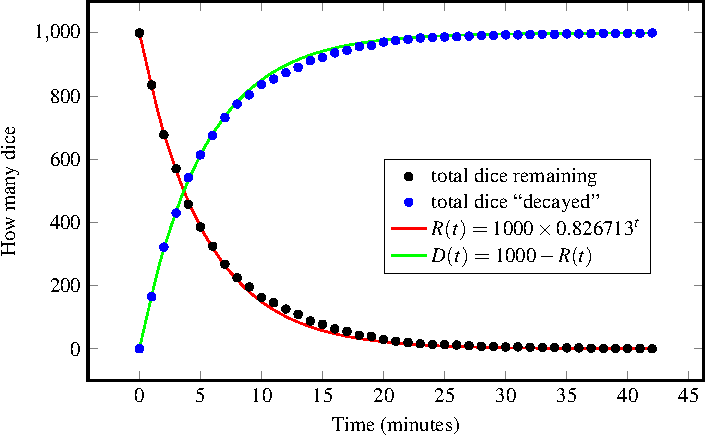
\includegraphics[scale=1.1]{image/11/radioactive-dice.pdf}
\caption{%%
  The decay of $1000$ ``radioactive'' dice.  The black graph
  represents the actual number of remaining ``undecayed'' dice after
  the elapse of the given number of minutes.  The red curve is a graph
  of \Equation{eqn:radioactive_dice_decay_constant_formula}, which
  predicts how many dice are yet to ``decay'' after $t$ minutes.
  Similarly, the blue graph represents the actual cumulative number of
  dice that have ``decayed'' after the elapse of a given number of
  minutes.  This number is predicted by
  \Equation{eqn:radioactive_dice_total_decayed}, which is represented
  by the green curve.  The experimental data are from
  \Table{tab:radioactive_dice}.
}
\label{fig:radioactive_dice}
\end{figure}

\solutionpart{subprob:radioactive_dice_cumulative_decayed}
See \Table{tab:radioactive_dice_cumulative_decayed} and
\Figure{fig:radioactive_dice}.

\begin{table}[!htbp]
\centering
\begin{tabular}{ccccrrcccc} \toprule
     &         & Running sum &           &&&      &         & Running sum &           \\
Time & Decayed & decayed     & Remaining &&& Time & Decayed & decayed     & Remaining \\\midrule
$0$  & $0$     & $0$         & $1000$    &&& $22$ & $4$     & $980$       & $20$      \\[4pt]
$1$  & $165$   & $165$       & $835$     &&& $23$ & $4$     & $984$       & $16$      \\[4pt]
$2$  & $157$   & $322$       & $678$     &&& $24$ & $2$     & $986$       & $14$      \\[4pt]
$3$  & $108$   & $430$       & $570$     &&& $25$ & $1$     & $987$       & $13$      \\[4pt]
$4$  & $112$   & $542$       & $458$     &&& $26$ & $1$     & $988$       & $12$      \\[4pt]
$5$  & $72$    & $614$       & $386$     &&& $27$ & $2$     & $990$       & $10$      \\[4pt]
$6$  & $61$    & $675$       & $325$     &&& $28$ & $2$     & $992$       & $8$       \\[4pt]
$7$  & $57$    & $732$       & $268$     &&& $29$ & $0$     & $992$       & $8$       \\[4pt]
$8$  & $43$    & $775$       & $225$     &&& $30$ & $2$     & $994$       & $6$       \\[4pt]
$9$  & $29$    & $804$       & $196$     &&& $31$ & $0$     & $994$       & $6$       \\[4pt]
$10$ & $33$    & $837$       & $163$     &&& $32$ & $1$     & $995$       & $5$       \\[4pt]
$11$ & $17$    & $854$       & $146$     &&& $33$ & $1$     & $996$       & $4$       \\[4pt]
$12$ & $20$    & $874$       & $126$     &&& $34$ & $0$     & $996$       & $4$       \\[4pt]
$13$ & $17$    & $891$       & $109$     &&& $35$ & $1$     & $997$       & $3$       \\[4pt]
$14$ & $21$    & $912$       & $88$      &&& $36$ & $0$     & $997$       & $3$       \\[4pt]
$15$ & $10$    & $922$       & $78$      &&& $37$ & $1$     & $998$       & $2$       \\[4pt]
$16$ & $15$    & $937$       & $63$      &&& $38$ & $1$     & $999$       & $1$       \\[4pt]
$17$ & $8$     & $945$       & $55$      &&& $39$ & $0$     & $999$       & $1$       \\[4pt]
$18$ & $12$    & $957$       & $43$      &&& $40$ & $0$     & $999$       & $1$       \\[4pt]
$19$ & $3$     & $960$       & $40$      &&& $41$ & $0$     & $999$       & $1$       \\[4pt]
$20$ & $11$    & $971$       & $29$      &&& $42$ & $1$     & $1000$      & $0$       \\[4pt]
$21$ & $5$     & $976$       & $24$ \\\bottomrule
\end{tabular}

\caption{%%
  This is the same as \Table{tab:radioactive_dice}, but with the
  addition of columns for the cumulative sum of dice that have
  ``decayed''.
}
\label{tab:radioactive_dice_cumulative_decayed}
\end{table}

\solutionpart{subprob:radioactive_dice_decay_constant}
The half-life of the ``radioactive'' dice is the amount of time
required for the dice to ``decay'' to half of their original quantity.
The initial quantity of dice is $1000$ and half of this is
$1000 / 2 = 500$ dice.  \Figure{fig:radioactive_dice} shows that the
dice required approximately $4$ minutes in order to ``decay'' to $500$
dice.  Thus the half-life of the dice is approximately $t_{1/2} = 4$
minutes.  Substitute the latter value into
\Equation{eqn:half_life_related_to_decay_rate} and you get
$4 = \frac{0.693147}{\lambda}$, which upon solving for $\lambda$
results in a constant decay rate of approximately
%%
\begin{align*}
\lambda
&=
\frac{0.693147}{4} \\[4pt]
&=
0.17328675.
\end{align*}
%%
Hence the decay factor is approximately
$b = 1 - \lambda \approx 0.826713$, rounded to six decimal places.
Note that you initially had $1000$ dice.  If $R(t)$ represents the
number of ``radioactive'' dice remaining after $t$ minutes, you can
write
%%
\begin{equation}
\label{eqn:radioactive_dice_decay_constant_formula}
R(t)
=
1000 \times 0.826713^t.
\end{equation}
%%
Then the total number $D(t)$ of dice that have ``decayed'' after $t$
minutes can be written as
%%
\begin{equation}
\label{eqn:radioactive_dice_total_decayed}
\begin{aligned}
D(t)
&=
1000 - R(t) \\[4pt]
&=
1000 - 1000 \times 0.826713^t \\[4pt]
&=
1000(1 - 0.826713^t).
\end{aligned}
\end{equation}
%%
The functions $R(t)$ and $D(t)$ are graphed in
\Figure{fig:radioactive_dice}.

\solutionpart{subprob:radioactive_dice_mean_decay_rate}
The mean of the relative decay factors is roughly $0.830929$, rounded
to six decimal places, so the decay factor can be estimated as
$b = 0.830929$.  If $M(t)$ represents the number of dice remaining
after $t$ minutes, you can write
%%
\begin{equation}
\label{eqn:radioactive_dice_mean_decay_rate}
M(t)
=
1000 \times 0.830929^t.
\end{equation}

\solutionpart{subprob:radioactive_dice_probability}
A die has six faces and the face with six pips is one among the six
faces.  Since each die is fair, after a roll the probability that the
top-most face of a die has six pips is $p = 1 / 6$ and you take this
as the probability that a die will ``decay''.  The probability $q$
that a die will not decay is $q = 1 - p$, which can also be written as
$q = 1 - \frac{1}{6}$ and simplifies to $q = 5 / 6$.  Given a large
number of dice, the probability of $q = 5 / 6$ is the same as the
proportion of dice that will remain ``undecayed'' during the next unit
of time.  That is, the probability of $q = 5 / 6$ is also the decay
factor, which means that $p = 1 / 6$ is the decay rate.  If $P(t)$
represents the number of dice remaining after $t$ minutes, you can
write
%%
\begin{equation}
\label{eqn:radioactive_dice_probability}
P(t)
=
1000
\times
\parenthesis*{\frac{5}{6}}^t.
\end{equation}

\begin{figure}[!htbp]
\centering
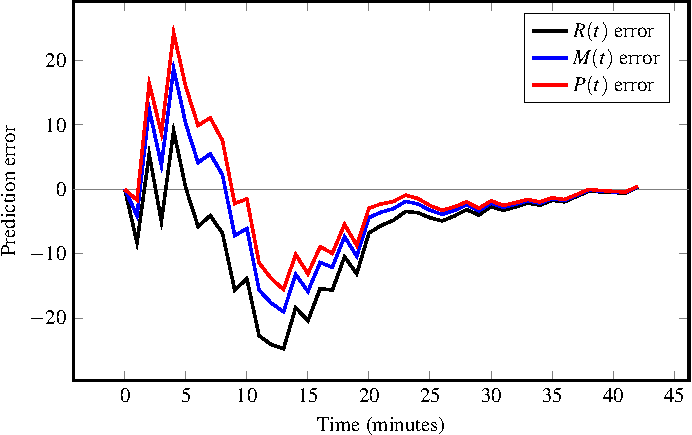
\includegraphics[scale=1.1]{image/11/radioactive-dice-error.pdf}
\caption{%%
  The errors of the functions
  $R(t)$~(\Equation{eqn:radioactive_dice_decay_constant_formula}),
  $M(t)$~(\Equation{eqn:radioactive_dice_mean_decay_rate}), and
  $P(t)$~(\Equation{eqn:radioactive_dice_probability}).  Let
  $\tuple{\tau}{\rho}$ be a data point from
  \Table{tab:radioactive_dice}, where $\tau$ denotes time in minutes
  and $\rho$ represents the number of dice remaining after $\tau$
  minutes.  The error of the function $R(t)$ at time $t = \tau$ is
  defined as the difference $R(\tau) - \rho$.  Furthermore, the error
  of $R(t)$ is the error of $R(t)$ for time $t = \seq{1}{2}{42}$.  The
  errors of $M(t)$ and $P(t)$ are similarly defined.
}
\label{fig:radioactive_dice_errors}
\end{figure}

\solutionpart{subprob:radioactive_dice_error_analysis}
\Figure{fig:radioactive_dice_errors} shows the errors of the functions
defined by
equations~\eqref{eqn:radioactive_dice_decay_constant_formula},
\eqref{eqn:radioactive_dice_mean_decay_rate}, and
\eqref{eqn:radioactive_dice_probability}.  Note the horizontal line
through the origin.  If an error value is above this line, then the
corresponding function overestimates a data point.  Similary, when an
error value is below the horizontal line, the corresponding function
underestimates a data point.  If an error value lies on the line, then
the corresponding function perfectly predicts the data point.  From
time $t = 1$ up to approximately $t = 8$, all three functions seem to
overestimate the experimental data.  The situation is reversed from
$t = 9$ up to approximately $t = 40$, a time interval during which the
functions underestimate the experimental data.  When the three
functions overestimate the data, $R(t)$ gives estimates that are
closer to zero than the other two functions.  However, when the
functions underestimate the data, $P(t)$ yields estimates that are
closer to zero than the other two functions.
\Figure{fig:radioactive_dice_errors} shows that overall $P(t)$ seems
to be better than the other two functions at modelling the data in
\Table{tab:radioactive_dice}.  This observation is confirmed by the
fact that of the root mean square errors of the three functions,
$P(t)$ has the lowest RMS error at $7.890036$, rounded to six decimal
places.
\end{solution}
}{}

\begin{table}[!htbp]
\centering
\begin{tabular}{cccccccccccccc}                                                                        \toprule
$\degreec{t}$ & Pressure &&& $\degreec{t}$ & Pressure &&& $\degreec{t}$ & Pressure &&& $\degreec{t}$ & Pressure \\\midrule
$0$           & $4.579$  &&& $26$          & $25.209$ &&& $52$          & $102.09$ &&& $78$          & $327.30$ \\[4pt]
$1$           & $4.926$  &&& $27$          & $26.739$ &&& $53$          & $107.20$ &&& $79$          & $341.00$ \\[4pt]
$2$           & $5.294$  &&& $28$          & $28.349$ &&& $54$          & $112.51$ &&& $80$          & $355.10$ \\[4pt]
$3$           & $5.685$  &&& $29$          & $30.043$ &&& $55$          & $118.04$ &&& $81$          & $369.70$ \\[4pt]
$4$           & $6.101$  &&& $30$          & $31.824$ &&& $56$          & $123.80$ &&& $82$          & $384.90$ \\[4pt]
$5$           & $6.543$  &&& $31$          & $33.695$ &&& $57$          & $129.82$ &&& $83$          & $400.60$ \\[4pt]
$6$           & $7.013$  &&& $32$          & $35.663$ &&& $58$          & $136.08$ &&& $84$          & $416.80$ \\[4pt]
$7$           & $7.513$  &&& $33$          & $37.729$ &&& $59$          & $142.60$ &&& $85$          & $433.60$ \\[4pt]
$8$           & $8.045$  &&& $34$          & $39.898$ &&& $60$          & $149.38$ &&& $86$          & $450.90$ \\[4pt]
$9$           & $8.609$  &&& $35$          & $42.175$ &&& $61$          & $156.43$ &&& $87$          & $468.70$ \\[4pt]
$10$          & $9.209$  &&& $36$          & $44.563$ &&& $62$          & $163.77$ &&& $88$          & $487.10$ \\[4pt]
$11$          & $9.844$  &&& $37$          & $47.067$ &&& $63$          & $171.38$ &&& $89$          & $506.10$ \\[4pt]
$12$          & $10.518$ &&& $38$          & $49.692$ &&& $64$          & $179.31$ &&& $90$          & $525.76$ \\[4pt]
$13$          & $11.231$ &&& $39$          & $52.442$ &&& $65$          & $187.54$ &&& $91$          & $546.05$ \\[4pt]
$14$          & $11.987$ &&& $40$          & $55.324$ &&& $66$          & $196.09$ &&& $92$          & $566.99$ \\[4pt]
$15$          & $12.788$ &&& $41$          & $58.340$ &&& $67$          & $204.96$ &&& $93$          & $588.60$ \\[4pt]
$16$          & $13.634$ &&& $42$          & $61.500$ &&& $68$          & $214.17$ &&& $94$          & $610.90$ \\[4pt]
$17$          & $14.530$ &&& $43$          & $64.800$ &&& $69$          & $223.73$ &&& $95$          & $633.90$ \\[4pt]
$18$          & $15.477$ &&& $44$          & $68.260$ &&& $70$          & $233.70$ &&& $96$          & $657.62$ \\[4pt]
$19$          & $16.477$ &&& $45$          & $71.880$ &&& $71$          & $243.90$ &&& $97$          & $682.07$ \\[4pt]
$20$          & $17.535$ &&& $46$          & $75.650$ &&& $72$          & $254.60$ &&& $98$          & $707.27$ \\[4pt]
$21$          & $18.650$ &&& $47$          & $79.600$ &&& $73$          & $265.70$ &&& $99$          & $733.24$ \\[4pt]
$22$          & $19.827$ &&& $48$          & $83.710$ &&& $74$          & $277.20$ &&& $100$         & $760.00$ \\[4pt]
$23$          & $21.068$ &&& $49$          & $88.020$ &&& $75$          & $289.10$                              \\[4pt]
$24$          & $22.387$ &&& $50$          & $92.510$ &&& $76$          & $301.40$                              \\[4pt]
$25$          & $23.756$ &&& $51$          & $97.200$ &&& $77$          & $314.10$                              \\\bottomrule
\end{tabular}

\caption{%%
  The vapour pressure of water as temperature increases.  Temperature
  is measured in degrees Celsius~($\degreec{}$) and the vapour
  pressure of water is measured in millimetre of mercury~(mm Hg).  The
  given vapour pressures cover only the case where water is in contact
  with its own vapour.  Data are taken from the following book:
  J.~G.~Speight~(editor). \emph{Lange's Handbook of Chemistry}. 16-th
  edition, McGraw-Hill, 2005, pp.1.224--1.225.
}
\label{tab:water_vapour_pressure}
\end{table}

\item Suppose you put water in a container and then seal the
  container.  As water evaporates inside the closed container, a layer
  of vapour forms above the water and this layer of vapour exerts
  pressure on the container.  As temperature increases so does the
  pressure, which explains the ``hiss'' sound when you open a sealed
  bottle of water.  \Table{tab:water_vapour_pressure} shows the vapour
  pressures of water between the temperatures of $\degreec{0}$ and
  $\degreec{100}$.
  %%
  \begin{packedenum}
  \item\label{subprob:water_mean_growth_factor}
    Graph the data in \Table{tab:water_vapour_pressure} as a scatter
    plot.  Assume that the data in \Table{tab:water_vapour_pressure}
    follow an exponential growth model.  Starting from $\degreec{1}$
    onwards, define the \emph{relative pressure growth} as the vapour
    pressure for the current temperature divided by the vapour
    pressure for the previous temperature.  Calculate the mean of all
    the relative pressure growths and let the result be an estimate of
    the growth factor of the vapour pressure of water.  Derive a
    formula to model the increase in the vapour pressure of water as
    temperature rises.  Graph your formula together with the given
    data set.  What do you notice?

  \item\label{subprob:water_Wikipedia_formula}
    The following is a simple exponential model of the data in
    \Table{tab:water_vapour_pressure}:\footnote{
      The formula is from the following website:
      \url{https://web.archive.org/web/20180504010448/https://en.wikipedia.org/wiki/Vapour_pressure_of_water},
      accessed 2018-05-04.
    }
    %%
    \begin{equation}
    \label{eqn:vapour_pressure_Wikipedia_formula}
    g(t)
    =
    \exp{
      20.386
      -
      \frac{5132}{273.15 + t}
    }.
    \end{equation}
    %%
    Here an expression such as $e^{\alpha + \beta}$ is also written as
    $\exp{\alpha + \beta}$.  Graph
    \Equation{eqn:vapour_pressure_Wikipedia_formula} together with the
    graph from \Part{subprob:water_mean_growth_factor}.  What do you
    notice?

  \item\label{subprob:vapour_pressure_Tetens}
    The \emph{Tetens equation}\footnote{
      See page~13 of the following book:
      J.~L.~Monteith and M.~H.~Unsworth.
      \emph{Principles of Environmental Physics: Plants, Animals, and
        the Atmosphere}. 4-th edition, Academic Press, 2013.
    }
    is one of the better formulae for approximating the vapour
    pressure of water.  If $T(t)$ represents the vapour
    pressure~(mm~Hg) of water at a temperature of $\degreec{t}$, then
    the Tetens equation can be written as
    %%
    \begin{equation}
    \label{eqn:vapour_pressure_Tetens}
    T(t)
    =
    7.500638 \times 0.61078
    \exp{
      \frac{
        17.27t
      }{
        237.3 + t
      }
    }.
    \end{equation}
    %%
    The factor of $7.500638$ ensures that the result of the Tetens
    equation is in units of mm~Hg.  Otherwise the result of the Tetens
    equation would be in units of kilopascals~(kPa), where one~kPa is
    approximately $7.500638$~mm~Hg.  Graph the Tetens
    \Equation{eqn:vapour_pressure_Tetens} together with the graph
    from \Part{subprob:water_Wikipedia_formula}.  What do you notice?

  \item\label{subprob:vapour_pressure_Buck}
    For temperatures greater than $\degree{0}$C, Arden Buck\footnote{
      See the paper at
      \url{https://doi.org/10.1175/1520-0450(1981)020<1527:NEFCVP>2.0.CO;2}
      and the document at
      \url{https://web.archive.org/web/20180504021107/http://www.hygrometers.com/wp-content/uploads/CR-1A-users-manual-2009-12.pdf},
      accessed 2018-05-04.
    }
    developed the following formula to model the vapour pressure
    $B(t)$ of water at $\degree{t}$C:
    %%
    \begin{equation}
    \label{eqn:vapour_pressure_Buck}
    \begin{aligned}
    B(t)
    &=
    7.500638 \times 0.61121 \\[4pt]
    \amptab
    \times
    \exp{
      \frac{t}{257.14 + t}
      \parenthesis*{
        18.678 - \frac{t}{234.5}
      }
    }.
    \end{aligned}
    \end{equation}
    %%
    Similar to the Tetens equation, the factor of $7.500638$ ensures
    that the Buck equation gives results in units of mm~Hg.  Graph the
    Buck \Equation{eqn:vapour_pressure_Buck} together with the graph
    from \Part{subprob:vapour_pressure_Tetens}.  What do you notice?

  \item\label{subprob:vapour_pressure_RMS_error}
    For each observed pressure number in
    \Table{tab:water_vapour_pressure}, calculate the squared error
    that results from using each of
    equations~\eqref{eqn:vapour_pressure_Wikipedia_formula},
    \eqref{eqn:vapour_pressure_Tetens},
    and~\eqref{eqn:vapour_pressure_Buck} to predict the vapour
    pressure at the given temperature.  Graph the temperatures versus
    the squared errors.  Use the graph to identify which of the above
    three equations is better at modelling vapour pressure for which
    range of temperatures.  Use the root mean square error~(i.e.~the
    RMS error) to explain which one of the three equations is better
    at modelling the data in \Table{tab:water_vapour_pressure}.
  \end{packedenum}
\ifbool{showSolution}{
\begin{solution}
\solutionpart{subprob:water_mean_growth_factor}
Let $a = 4.579$~mm~Hg be the initial vapour pressure.  The mean of all
the relative pressure growths is approximately $b = 1.0525$, rounded
to four decimal places.  If $f(t)$ represents the vapour
pressure~(mm~Hg) of water at a temperature of $\degreec{t}$, then you
can write $f(t)$ as
%%
\begin{equation}
\label{eqn:water_mean_growth_factor}
f(t)
=
4.579 \times 1.0525^t.
\end{equation}
%%
The latter equation is graphed in \Figure{fig:water_vapour_pressure}
together with the data from \Table{tab:water_vapour_pressure}.  The
figure shows that \Equation{eqn:water_mean_growth_factor} tends to
underestimate the vapour pressure of water, especially within the
region of $\degreec{20}$ to $\degreec{100}$.

\begin{figure}[!htbp]
\centering
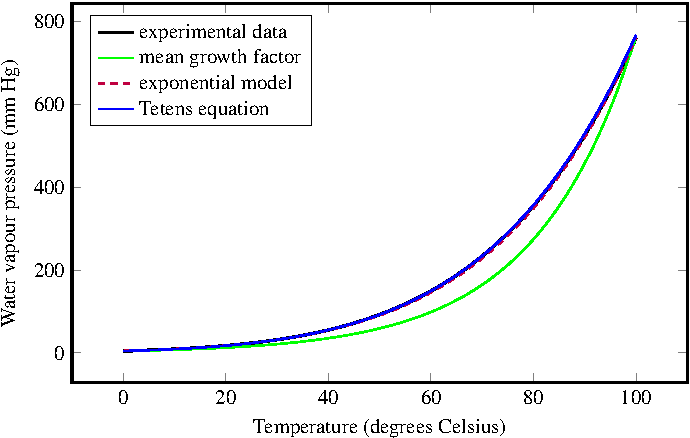
\includegraphics[scale=1.1]{image/11/vapour-pressure.pdf}
\caption{%%
  The vapour pressure of water as a function of temperature.  Vapour
  pressure is measured in millimetre of mercury and temperature is
  measured in degrees Celsius.  The experimental data are from
  \Table{tab:water_vapour_pressure}.  The green curve is a graph of
  \Equation{eqn:water_mean_growth_factor}.  The dashed curve is a
  graph of \Equation{eqn:vapour_pressure_Wikipedia_formula}.  The blue
  curve is a graph of the Tetens
  \Equation{eqn:vapour_pressure_Tetens}.  The graph of the Buck
  \Equation{eqn:vapour_pressure_Buck} is not shown because it overlaps
  the curves for the experimental data and the Teten equation.
}
\label{fig:water_vapour_pressure}
\end{figure}

\solutionpart{subprob:water_Wikipedia_formula}
\solutionpart{subprob:vapour_pressure_Tetens}
\solutionpart{subprob:vapour_pressure_Buck}
\Figure{fig:water_vapour_pressure} compares the graphs of
\Equations{eqn:vapour_pressure_Wikipedia_formula}{eqn:water_mean_growth_factor}
and the Tetens \Equation{eqn:vapour_pressure_Tetens}.  Note that the
graph for the Buck \Equation{eqn:vapour_pressure_Buck} is not shown
because it overlaps with the graphs of
\Equation{eqn:vapour_pressure_Wikipedia_formula} and the Teten
equation.  The figure shows that
\Equation{eqn:vapour_pressure_Wikipedia_formula} is better suited to
modelling the given data set than is
\Equation{eqn:water_mean_growth_factor}.  The Tetens and Buck
equations and the exponential
model~\eqref{eqn:vapour_pressure_Wikipedia_formula} all seem to
overlap the experimental data, which clearly suggests that you require
another way to decide which one of the latter three equations is
better suited to modelling the given data set.

\begin{figure}[!htbp]
\centering
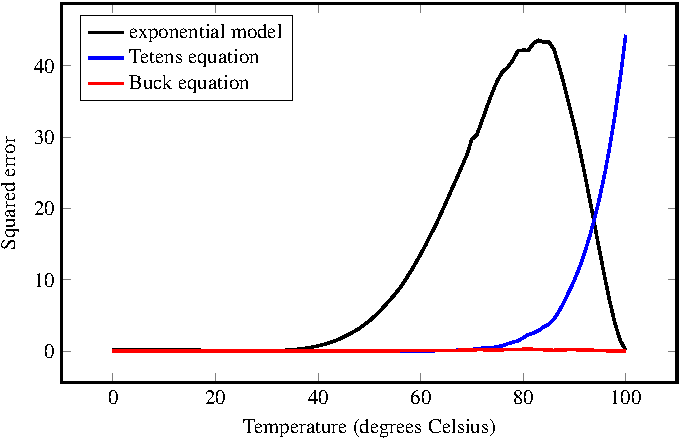
\includegraphics[scale=1.1]{image/11/vapour-pressure-squared-errors.pdf}
\caption{%%
  The squared errors of each of the exponential
  model~\eqref{eqn:vapour_pressure_Wikipedia_formula}, the Tetens
  \Equation{eqn:vapour_pressure_Tetens}, and the Buck
  \Equation{eqn:vapour_pressure_Buck}.
}
\label{fig:vapour_pressure_squared_errors}
\end{figure}

\solutionpart{subprob:vapour_pressure_RMS_error}
\Figure{fig:vapour_pressure_squared_errors} compares the squared
errors of the exponential
model~\eqref{eqn:vapour_pressure_Wikipedia_formula}, the Tetens
\Equation{eqn:vapour_pressure_Tetens}, and the Buck
\Equation{eqn:vapour_pressure_Buck}.  The figure shows that the
exponential \Equation{eqn:vapour_pressure_Wikipedia_formula} can be
used to model the vapour pressure of water when the
temperature $t$~($\degreec{}$) is within the range
$0 \leq t \leq 40$.  From $\degreec{40}$ onwards, the quality of the
prediction of \Equation{eqn:vapour_pressure_Wikipedia_formula}
deteriorates.  Similarly, the Tetens
\Equation{eqn:vapour_pressure_Tetens} can be used to predict vapour
pressure for temperatures~($\degreec{}$) within the range
$0 \leq t \leq 75$.  However, the quality of the prediction of the
Buck \Equation{eqn:vapour_pressure_Buck} does not seem to deteriorate
as the temperature increases from $\degreec{0}$ to $\degreec{100}$.
This is further confirmed by the fact that of the three equations, the
Buck equation has the lowest RMS error, namely~$0.2377$, rounded to
four decimal places.  Therefore you may conclude that the Buck
equation is better than the other two at modelling the data in
\Table{tab:water_vapour_pressure}.
\end{solution}
}{}

\begin{table}[!htbp]
\centering
\begin{tabular}{cc} \toprule
Hours & Observed \\\midrule
$0$   & $9.6$    \\[4pt]
$1$   & $18.3$   \\[4pt]
$2$   & $29.0$   \\[4pt]
$3$   & $47.2$   \\[4pt]
$4$   & $71.1$   \\[4pt]
$5$   & $119.1$  \\[4pt]
$6$   & $174.6$  \\[4pt]
$7$   & $257.3$  \\[4pt]
$8$   & $350.7$  \\[4pt]
$9$   & $441.0$  \\[4pt]
$10$  & $513.3$  \\[4pt]
$11$  & $559.7$  \\[4pt]
$12$  & $594.8$  \\[4pt]
$13$  & $629.4$  \\[4pt]
$14$  & $640.8$  \\[4pt]
$15$  & $651.1$  \\[4pt]
$16$  & $655.9$  \\[4pt]
$17$  & $659.6$  \\[4pt]
$18$  & $661.8$  \\\bottomrule
\end{tabular}

\caption{%%
  The observed population size in an experimental colony of yeast.
  The data are due to T.~Carlson, published in~1913.  The column for
  hours lists the numbers of hours that the population had been
  allowed to grow.  The column for observed numbers lists the counts
  of the number of yeast cells that were found in the colony after a
  given number of hours.
}
\label{tab:yeast}
\end{table}

\item In many situations, the exponential growth model as described
  in \Section{sec:exponential_growth} can produce results that do not
  make sense, are absurd, or just plain wrong.  Given a population of
  a particular animal, e.g.~rabbits, common sense tells you that the
  population number cannot keep on increasing larger and larger.  One
  simple reason is that the environment within which the rabbits live
  do not have an unlimited supply of food.  An implication is that
  there must be a point at which the population cannot grow any larger
  because there would not be enough food for every rabbit.  In
  situations of limited resources, you can use a more realistic model
  due to Pierre Fran\c{c}ois Verhulst called the \emph{logistic model}
  to investigate the growth of a population subject to the limited
  resources of its environment.  Let $A$ be the initial population
  size and suppose that the environment within which the population
  survives can support a maximum population size of $K$.  Assume that
  the population grows at a constant rate~(written as a decimal) of
  $r$ per unit time.  If $P(t)$ represents the population size at time
  $t$, then you write the population number as the logistic equation
  %%
  \begin{equation}
  \label{eqn:logistic_equation}
  P(t)
  =
  \frac{
    AK
  }{
    A + (K - A) \cdot e^{-rt}
  }.
  \end{equation}
  %%
  \begin{packedenum}
  \item\label{subprob:yeast_data_mean_growth_factor}
    \Table{tab:yeast} shows the population numbers of an experimental
    colony of yeast that had been allowed to grow for up to $18$
    hours.  Starting from the first hour onwards, define the
    \emph{hourly growth factor} as the observed number of yeast cells
    for the current hour divided by the observed number of yeast cells
    in the previous hour.  Calculate the mean of the hourly growth
    factors; call this the \emph{mean growth factor}.  Assuming that
    the yeast population grew according to an exponential model, use
    the mean growth factor to derive a formula for the number $Y(t)$
    of yeast cells after $t$ hours have elapsed.  Produce a graph of
    the experimental data in \Table{tab:yeast}.  On the same set of
    axes, graph your formula $Y(t)$.  What do you notice?

  \item\label{subprob:yeast_quintic_polynomial}
    Suppose you model the data in \Table{tab:yeast} as a polynomial of
    degree five.  A polynomial of degree five is also called a
    \emph{quintic polynomial}.  If $f(t)$ represents the number of
    yeast cells after $t$ hours, then write $f(t)$ as the quintic
    polynomial
    %%
    \begin{equation}
    \label{eqn:yeast_quintic_polynomial}
    \begin{aligned}
    f(t)
    &=
    0.0052x^5 - 0.2069x^4 + 2.3331x^3 \\[4pt]
    \amptab-
    3.2478x^2 + 2.6845x + 14.2567.
    \end{aligned}
    \end{equation}
    %%
    On the same set of axes, graph
    \Equation{eqn:yeast_quintic_polynomial}, your formula
    from \Part{subprob:yeast_data_mean_growth_factor}, and the data
    from \Table{tab:yeast}.  What do you notice?

  \item\label{subprob:yeast_logistic}
    In~1927, Raymond Pearl used the logistic
    \Equation{eqn:logistic_equation} to model the data in
    \Table{tab:yeast}.\footnote{
      See the following paper for further details:
      \url{https://doi.org/10.1086/394288}.
    }
    If $P(t)$ represents the number of yeast cells after $t$ hours,
    Pearl found that the data in the table can be modelled as
    %%
    \begin{equation}
    \label{eqn:yeast_Pearl_logistic_equation}
    P(t)
    =
    \frac{
      665
    }{
      1 + e^{4.1896 - 0.5355t}
    }.
    \end{equation}
    %%
    Graph \Equation{eqn:yeast_Pearl_logistic_equation} on the same set
    of axes as the graph in \Part{subprob:yeast_quintic_polynomial}.
    What do you notice?  By using the root mean square error~(i.e.~the
    RMS error), explain which one of the equations
    from \Part{subprob:yeast_data_mean_growth_factor},
    \Part{subprob:yeast_quintic_polynomial}, and
    \Equation{eqn:yeast_Pearl_logistic_equation} is more suitable at
    modelling the data in \Table{tab:yeast}.
  \end{packedenum}
\ifbool{showSolution}{
\begin{solution}
\solutionpart{subprob:yeast_data_mean_growth_factor}
\Table{tab:yeast_hourly_growth_factors} shows the hourly growth
factors of the experimental colony of yeast.  Using the hourly growth
factors, the mean growth factor is calculated to be $1.2937$, rounded
to four decimal places.  Suppose that the yeast population grew
according to an exponential model.  Let $a = 9.6$ yeast cells be the
initial population and let $b = 1.2937$ be the growth factor.  If
$Y(t)$ represents the population size after $t$ hours, then the
population size can be written as
%%
\begin{equation}
\label{eqn:yeast_exponential_model}
Y(t)
=
9.6 \times 1.2937^t.
\end{equation}
%%
\Figure{fig:yeast_data_versus_models} shows a graph of the exponential
model~\eqref{eqn:yeast_exponential_model} fitted to the experimental
data given in \Table{tab:yeast}.  The figure clearly shows that an
exponential growth model is not appropriate for the data set under
consideration.

\begin{table}[!htbp]
\centering
\begin{tabular}{ccc}               \toprule
Hour  & Observed & Growth factor \\\midrule
$0$   & $9.6$    & ---           \\
$1$   & $18.3$   & $1.9063$      \\
$2$   & $29.0$   & $1.5847$      \\
$3$   & $47.2$   & $1.6276$      \\
$4$   & $71.1$   & $1.5064$      \\
$5$   & $119.1$  & $1.6751$      \\
$6$   & $174.6$  & $1.4660$      \\
$7$   & $257.3$  & $1.4737$      \\
$8$   & $350.7$  & $1.3630$      \\
$9$   & $441.0$  & $1.2575$      \\
$10$  & $513.3$  & $1.1639$      \\
$11$  & $559.7$  & $1.0904$      \\
$12$  & $594.8$  & $1.0627$      \\
$13$  & $629.4$  & $1.0582$      \\
$14$  & $640.8$  & $1.0181$      \\
$15$  & $651.1$  & $1.0161$      \\
$16$  & $655.9$  & $1.0074$      \\
$17$  & $659.6$  & $1.0056$      \\
$18$  & $661.8$  & $1.0033$      \\\bottomrule
\end{tabular}

\caption{%%
  The hourly growth factors of an experimental colony of yeast.  The
  growth factors have been rounded to four decimal places.  The
  experimental data are from \Table{tab:yeast}.
}
\label{tab:yeast_hourly_growth_factors}
\end{table}

\begin{figure}[!htbp]
\centering
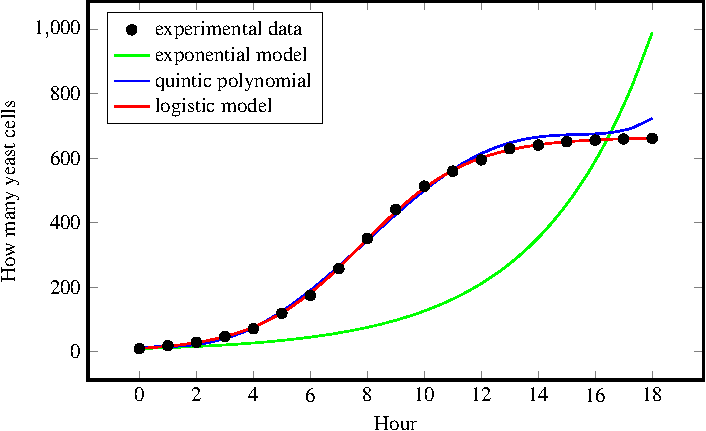
\includegraphics[scale=1.1]{image/11/yeast.pdf}
\caption{%%
  The observed yeast population size versus the number of yeast cells
  as predicted by the exponential
  function~\eqref{eqn:yeast_exponential_model}, the quintic
  polynomial~\eqref{eqn:yeast_quintic_polynomial}, and the logistic
  function~\eqref{eqn:yeast_Pearl_logistic_equation}.  The
  experimental data are from \Table{tab:yeast}.  The exponential
  growth model is clearly unsuitable for the given data set.
}
\label{fig:yeast_data_versus_models}
\end{figure}

\solutionpart{subprob:yeast_quintic_polynomial}
\Figure{fig:yeast_data_versus_models} shows a comparison of the
experimental data given in \Table{tab:yeast}, the exponential
model~\eqref{eqn:yeast_exponential_model}, and the quintic
polynomial~\eqref{eqn:yeast_quintic_polynomial}.  The figure clearly
shows that the quintic polynomial is better than the exponential
function at modelling the given experimental data.

\begin{table}[!htbp]
\centering
\begin{tabular}{crrrrcrrr} \toprule
      &          & \multicolumn{3}{c}{Models} && \multicolumn{3}{c}{Squared error} \\
  \cmidrule{3-5} \cmidrule{7-9}
Hours & Observed & Exponential & Quintic & Logistic && Exponential  & Quintic    & Logistic \\\midrule
$0$   & $9.6$    & $9.6$       & $14.3$  & $9.9$    && $0.000$      & $21.685$   & $0.106$  \\[4pt]
$1$   & $18.3$   & $12.4$      & $15.8$  & $16.8$   && $34.580$     & $6.127$    & $2.313$  \\[4pt]
$2$   & $29.0$   & $16.1$      & $22.2$  & $28.2$   && $167.259$    & $46.850$   & $0.705$  \\[4pt]
$3$   & $47.2$   & $20.8$      & $40.6$  & $46.7$   && $697.697$    & $43.846$   & $0.244$  \\[4pt]
$4$   & $71.1$   & $26.9$      & $74.7$  & $76.0$   && $1954.443$   & $13.008$   & $24.071$ \\[4pt]
$5$   & $119.1$  & $34.8$      & $125.1$ & $120.1$  && $7108.383$   & $35.512$   & $1.035$  \\[4pt]
$6$   & $174.6$  & $45.0$      & $189.7$ & $181.9$  && $16794.543$  & $227.566$  & $53.612$ \\[4pt]
$7$   & $257.3$  & $58.2$      & $264.8$ & $260.3$  && $39631.027$  & $56.082$   & $9.202$  \\[4pt]
$8$   & $350.7$  & $75.3$      & $345.4$ & $348.2$  && $75831.322$  & $28.602$   & $6.339$  \\[4pt]
$9$   & $441.0$  & $97.4$      & $425.8$ & $433.9$  && $118027.899$ & $232.282$  & $50.546$ \\[4pt]
$10$  & $513.3$  & $126.1$     & $500.4$ & $506.9$  && $149948.138$ & $165.851$  & $40.477$ \\[4pt]
$11$  & $559.7$  & $163.1$     & $564.4$ & $562.4$  && $157295.542$ & $22.096$   & $7.069$  \\[4pt]
$12$  & $594.8$  & $211.0$     & $614.0$ & $600.8$  && $147305.530$ & $369.881$  & $36.098$ \\[4pt]
$13$  & $629.4$  & $273.0$     & $647.6$ & $625.9$  && $127045.558$ & $329.437$  & $12.553$ \\[4pt]
$14$  & $640.8$  & $353.1$     & $665.7$ & $641.5$  && $82750.889$  & $620.593$  & $0.509$  \\[4pt]
$15$  & $651.1$  & $456.9$     & $672.4$ & $651.0$  && $37732.541$  & $454.508$  & $0.003$  \\[4pt]
$16$  & $655.9$  & $591.0$     & $675.3$ & $656.8$  && $4208.301$   & $378.159$  & $0.741$  \\[4pt]
$17$  & $659.6$  & $764.6$     & $686.6$ & $660.2$  && $11027.872$  & $726.885$  & $0.305$  \\[4pt]
$18$  & $661.8$  & $989.2$     & $723.1$ & $662.2$  && $107178.131$ & $3763.688$ & $0.125$  \\\bottomrule
\end{tabular}

\caption{%%
  A comparison of three models of the data in \Table{tab:yeast}.  The
  first is the exponential
  function~\eqref{eqn:yeast_exponential_model}, the second is the
  quintic polynomial~\eqref{eqn:yeast_quintic_polynomial}, and the
  third is the logistic
  function~\eqref{eqn:yeast_Pearl_logistic_equation}.  The predictions
  of these models have been rounded to one decimal place.  Also shown
  are the squared errors of each model.  These errors have been
  rounded to three decimal places.  Note that most numbers have been
  rounded so as to fit the table.  However, you should avoid rounding
  any intermediate results.
}
\label{tab:yeast_compare_models}
\end{table}

\solutionpart{subprob:yeast_logistic}
\Figure{fig:yeast_data_versus_models} shows a comparison of three
functions for modelling the experimental data given in
\Table{tab:yeast}.  Of the three functions, the logistic function
seems to be better than the other two at modelling the data.  This
observation is also confirmed by the root mean square errors of the
three functions.  \Table{tab:yeast_compare_models} shows the squared
errors of each of the three models.  Using these squared errors the
exponential, quintic, and logistic functions have, respectively, RMS
errors of $238.9384$, $19.9244$, and $3.5986$.  This clearly shows
that the logistic function is better suited to modelling the given
data than either of the exponential or quintic functions.
\end{solution}
}{}
\end{problem}

\end{document}
